\newpage

\section{Time Schedule for the Project}
\begin{center}
    \includegraphics[width=\linewidth]{Bilder/gannt1.jpg}
\end{center}

\section{Abstract}
As the usage of EVs increases globally, efficient deployment of charging station infrastructure has become a critical component of sustainable urban mobility.Determining optimal locations for EV charging stations is crucial for minimizing infrastructure costs and maximizing operational efficiency. Policymakers can leverage data-driven approaches to make informed decisions, ensuring that charging infrastructure meets demand effectively while remaining cost-efficient. This paper focuses on and uses the methods of AI to solve the problem of efficient EV charging station deployment. Utilizing open-access data sources, such as Berlin Open Data, the research analyzes spatial patterns, utilization rates, heatmaps and key factors influencing the efficiency of the locations of charging stations, including geographical, social, and economic determinants. AI methodologies are also weighed against each other to find that supervised learning with neural networks is the most optimal AI methodology for the problem at hand. However, due to data limitations, a real life example is not possible to be built at the time of publishing. A pre-trained supervised learning model developed by Jayanath et al.\cite{Jayanath2024} was used to give insight to optimal EV charger locations but was found to be very biased towards traffic volume. Then an unsupervised learning model was built to find the underlying patterns in existing infrastructure. Using Analytic Hierarchy Process to rank patterns in infrastructure it was made possible to find and visualize the most optimal EV charger locations in Berlin.

\textbf{Keywords: }Electric vehicle charging station deployment, Spatial data analysis, GIS systems, Berlin, Urban planning, Artifical intelligence, Machine learning

\clearpage  

\section{Introduction}

\begin{figure}[hbt!]
\begin{center}
\includegraphics[width=0.75\textwidth]{Bilder/[1].png}
\caption{Total U.S Greenhouse Gas Emissions by Economic Sector Including Electricity End-Use Indirect Emissions. \cite{EPA_GHG}}\label{fig:[1]}
\end{center}
\end{figure}
Burning fossil fuels for transportation, including cars, trucks, ships, and planes, produces greenhouse gas emissions. Transportation uses mostly petroleum-based fuel, primarily gasoline and diesel, which cause direct emissions. It is also the second largest direct and indirect greenhouse gas emissions source, and the third largest comes from industry. To process raw materials into finished goods or products, industry also needs energy from burning fossil fuels and which causes greenhouse gas emissions. It is shown above that industry highly contributed of U.S. greenhouse gas emissions. Burning natural gas or petroleum for electric power is less carbon-intensive than coal. In the United States, coal was responsible for 55\% of the sector’s $\text{CO}_2$ emissions, but only 20\% of the electricity generated from coal was generated in 2022 \cite{EPA_GHG}. one of the important steps for more national energy security, less reliance on imported fossil fuels, and an increasingly energy-sustainable future is introducing electric vehicles. Countries can embark on a cleaner transportation future powered by innovation, resilience, and environmental responsibility by working together and collaborating with industry to build the infrastructure needed to achieve that \cite{Cyberswitching_Independence}. 
\\

\begin{figure}[hbt!]
\begin{center}
\includegraphics[width=0.75\textwidth]{Bilder/[2].png}
\caption{Lifecycle Greenhouse Gases. \cite{EPA_Myths}}\label{fig:[3]}
\end{center}
\end{figure}

In the production of electric vehicles, battery manufacturing is also needed as an important part of it, which is accused of still causing pollution. Throughout the lifetime of electric vehicles, starting from manufacturing then charging and driving, electric vehicles are still calculated to be less in the production of greenhouse gas emissions compared to internal combustion engine vehicles, which can be seen in the following figure where it can be seen a very clear comparison, namely where the gas car during its use contributes 74\% in its lifecycle. Unlike gasoline cars, electric vehicles do not produce greenhouse gas emissions during use. Compared to internal combustion engine vehicles (\gls{ICEV}s), electric vehicles (\gls{EV}s) have a considerable advantage in terms of energy efficiency. For example, EVs convert 87\%–91\% of energy from batteries whereas ICEVs can only convert 16–25\% of gasoline \cite{EPA_Myths}. Despite the significant advantages that EVs have and their worldwide implementation, the availability and accessibility of EV charging stations are issues, and the cost of batteries is also another obstacle that needs to be faced since batteries are one of the important parts of EVs. Even though installing charging infrastructure at home is possible and inexpensive (ca. 200 EUR), it still doesn't compare to the charging speed of not charging stations. Another problem in introducing electric vehicles is consumer acceptance or customer readiness to adopt EVs due to many considerations, such as performance concerns or, as mentioned above, the availability and accessibility of charging infrastructure. There are also other technical issues such as standardization, Safety requirements for recharging/discharging places, Charging cable at the car or at the recharging station, Periodic inspections and maintenance of recharging places, Cross-national compatibility (re-charging abroad should not be different to recharging at home). Several approaches to help where to place EV charging stations in urban areas have been proposed in response to this issue. Electric vehicles can also be considered to be more environmentally friendly, which can help reduce contributions to greenhouse gas emissions and local air pollution \cite{Ajanovic2014}.
\\

\begin{figure}[htbp]
\begin{center}
\includegraphics[width=0.75\textwidth]{Bilder/[11].jpg}
\caption{Development of the global sales market for EVs between 2012 and 2022. \cite{Fraunhofer_Blog}}\label{fig:[11]}
\end{center}
\end{figure}


The EV market has seen more consumers and businesses experiencing rapid expansion as companies and people choose EVs to reduce their carbon footprint and take advantage of financial incentives. Despite the market growth, the efficiency and management of charging infrastructure is still an issue. One of the solutions for this scene is artificial intelligence (AI), which can be promising in optimizing strategies for the deployment of EV charging stations \cite{DunamisCharge_AI}.AI can play a major role in maximizing the advantages of electric mobility while searching for a solution to overcome the problem of energy infrastructure \cite{AfaxPower_AI}. with the help of AI algorithms, it is possible to identify optimal EV charging station deployment and distribution by collecting and analyzing specific data such as traffic patterns, user behaviour, and geographic features. AI will become more important in the future, while the EV infrastructure expands further. To ensure that the energy demand can be accommodated sustainably, AI algorithms can also pave the way to the integration with renewable energy sources, such as solar and wind power. This can lead to lower greenhouse gas emissions and a shift toward a more sustainable energy ecosystem \cite{EMobilityPlus_AI}. 
\\

\begin{figure}[H]
\begin{center}
\includegraphics[width=0.75\textwidth]{Bilder/[14].png}
\caption{3 Charging levels for EVs. \cite{EVChargingLevels}}\label{fig:[14]}
\end{center}
\end{figure}


The vehicle industry is experiencing rapid development with the emergence of many innovations, one of which is the three different EV charging levels with their objectives, even though these levels are suitable for all EV drivers. The vehicle industry is experiencing rapid development with the emergence of many innovations, one of which is the three different EV charging levels with their objectives, even though these levels are suitable for all EV drivers. Level 1 can be regarded as a basic wall plug. Level 1 EV charging has the slowest case speed, with a power rate of around 1.8kW to 2.4kW. For example, it takes 20 hours to get the capacity that can be used to travel 120 miles. Most public charging stations provide a level 2 charging station with a power rate of 3.6kW to 9.6kW, which is faster than the level 1 charging station. Rather than alternating current that is used for level 1 and level 2 charging station level 3 charging station uses direct current which can charge with high speed with power rate 25kW to 350kW. Due to the high cost and the inadequate electrical infrastructure, a level 3 charging station cannot be installed at home \cite{HowToGeekEVChargerLevels, EVChargingLevels}.

\section{Problem Definition}
The main focus of this project is the implementation of AI to optimize EV Charging station deployment in urban areas. This multi-objective problem has various key factors such as traffic flow, parking place, population density, and geographic features. Each key factor has issues that can lead to unideal deployment decisions. With the utilization of AI, it is possible to redefine the placement of EV charging stations in many ways through data analytics from the key factors despite the issues from each factor \cite{EVChargingSummit_AI}.
\subsection{Parking Availability}\label{sec:41}
As the introduction outlines, The EV market has seen more consumers and businesses experiencing rapid expansion. The adequate EV charging infrastructure continues to be one of the limitations for deploying an Urban EV transportation system, particularly in Asian cities with high population densities, such as Singapore, Hong Kong, and Shanghai.\cite{Wang2024} The demand for accessible and efficient EV charging stations is rapidly increasing as the global transition to EVs continues expanding. EV charging infrastructure placement is becoming dependent on residential and commercial parking places because parking lots are one of the most strategic places suitable for deploying EV charging stations due to their accessibility and convenience for EV drivers, although there are limited parking spaces  \cite{PilotEnergyStorage2024}.
\subsection{Traffic Flow}\label{sec:42}

\begin{figure}[H]
\begin{center}
\includegraphics[width=0.75\textwidth]{Bilder/[12].jpg}
\caption{Example of Charging Stations Based on Traffic Flow. \cite{TrafficFlowData}}\label{fig:[12]}
\end{center}
\end{figure}

Traffic flow plays a vital role in the optimal deployment of EV charging stations. Collecting other relevant data, such as the landscape of the roads and the mapping of specific areas, enables us to predict the areas with the most demand for charging stations, as EV owners are more likely to stop for charging when passing through this area, and slightly lower the traffic jam. Lowering traffic congestion can also be minimized by the optimal deployment of EV charging stations, where the EV owner can charge the vehicle rather than wasting time in traffic congestion  \cite{TrafficFlowData}.

\subsection{Energy Distribution}\label{sec:43}
Energy distribution can be included in the consideration for planning the deployment of EV charging stations. The challenges that will be faced in energy distribution are grid that can be suitable for each customer and every charging station has various energy or electricity capacity due to dependency on the demand at each charging station where the higher the demand the bigger the capacity required. At the same time, this will also cause problems with the cost of the right-sized electric vehicle supply equipment and maintaining the charging station  \cite{GridPlanning_EV}.


\section{Objectives}
The purpose of this project is to explore the use of AI methods for planning EV charging station deployment in urban areas through research and analysis of AI-based models and relevant data sources such as traffic flow, parking, and demographics. This project aims to determine the key factors influencing optimal EV charging station placement in urban areas. With the knowledge of specific factors, relevant data sources and estimates of necessary infrastructure for the future, it is possible to choose the most suitable AI methodologies for charging station deployment planning and compare the approach of AI-driven to traditional planning methods.

\section{Data}
\subsection{Turning the Motivation into Data}\label{sec:41}
\subsubsection{What the motivation is:}\label{sec:42}

A standard and publicly available data type is charger utilization rate. Charging stations have to first communicate with the EVs to start the energy transaction as specified by ISO 15118\cite{ISO15118} and charging times can be tracked. ISO 15118\cite{ISO15118} is a standard that was developed with the goal that allows for a secure and user-convenient way of charging EV’s while allowing the user mobility and providing stable and at the same time being stable and energy-efficient. \cite{Mueltin2018}.

As shown in this paper that is explaining the overview of ISO 15118 \cite{ISO15118} \cite{Mueltin2018}, and in the following table it illustrates the organization of the communication protocols between EV and charging stations in OSI (Open System Interconnection) layers.

Between two endpoints that are EVCC (EV Communication Controller) and SECC ( Supply Equipment Communication Controller), after the process of all the data that is to be used while charging is done, the communcation between two endpoints happens with either a charging cable or a wi-fi connection. 

\clearpage
Through the layer 7 (Application Layer), ISO 15118 logs the data such as:

\begin{table}[!hbt]
\hskip -0.85cm
\begin{tabular}{|c|c|c|cc|c|}
\hline
\begin{tabular}[c]{@{}c@{}}Application\\ OSI layer 7\end{tabular}   & \multirow{7}{*}{\begin{tabular}[c]{@{}c@{}}ISO 15118-1\\ \\ General \\ information\\ and use case \\ definition\\ \\ (merged with\\ contents of\\ ISO 15118-6\\ for second \\ edition)\end{tabular}} & \multirow{5}{*}{\begin{tabular}[c]{@{}c@{}}ISO 15118-2\\ \\ Network and \\ application\\ protocol\\ requirements\\ and\\ ISO 15118-20\\ 2nd generation\\ network and\\ application\\ protocol \\ requirements\end{tabular}} & \multicolumn{2}{c|}{\begin{tabular}[c]{@{}c@{}}Application layer messages\\ (V2G Message),\\ SDP (SECC Discovery\\ Protocol)\end{tabular}}                          & \multirow{5}{*}{\begin{tabular}[c]{@{}c@{}}ISO 15118-4\\ \\ Network and\\ application\\ protocol\\ conformance\\ tests\end{tabular}} \\ \cline{1-1} \cline{4-5}
\begin{tabular}[c]{@{}c@{}}Presentation \\ OSI layer 6\end{tabular} &                                                                                                                                                                                                      &                                                                                                                                                                                                                             & \multicolumn{2}{c|}{\begin{tabular}[c]{@{}c@{}}EXI (Efficient XML \\ Interchange)\end{tabular}}                                                                     &                                                                                                                                      \\ \cline{1-1} \cline{4-5}
\begin{tabular}[c]{@{}c@{}}Session\\ OSI layer 5\end{tabular}       &                                                                                                                                                                                                      &                                                                                                                                                                                                                             & \multicolumn{2}{c|}{\begin{tabular}[c]{@{}c@{}}V2GTP (Vehicle-to-Grid\\ Transfer Protocol)\end{tabular}}                                                            &                                                                                                                                      \\ \cline{1-1} \cline{4-5}
\begin{tabular}[c]{@{}c@{}}Transport \\ OSI layer 4\end{tabular}    &                                                                                                                                                                                                      &                                                                                                                                                                                                                             & \multicolumn{2}{c|}{\begin{tabular}[c]{@{}c@{}}UDP (User Datagram Protocol)\\ TCP (Transmission Control\\ Protocol),\\ TLS (Transport Layer Security)\end{tabular}} &                                                                                                                                      \\ \cline{1-1} \cline{4-5}
\begin{tabular}[c]{@{}c@{}}Network\\ OSI layer 3\end{tabular}       &                                                                                                                                                                                                      &                                                                                                                                                                                                                             & \multicolumn{2}{c|}{\begin{tabular}[c]{@{}c@{}}IP (Internet Protocol),\\ SLAAC,\\ DHCP\end{tabular}}                                                                &                                                                                                                                      \\ \cline{1-1} \cline{3-6} 
\begin{tabular}[c]{@{}c@{}}Data link\\ OSI layer 2\end{tabular}     &                                                                                                                                                                                                      & \multirow{2}{*}{ISO 15118-3}                                                                                                                                                                                                & \multicolumn{1}{c|}{\multirow{2}{*}{ISO 15118-5}}                                           & \multirow{2}{*}{ISO 15118-8}                                          & \multirow{2}{*}{ISO 15118-9}                                                                                                         \\ \cline{1-1}
\begin{tabular}[c]{@{}c@{}}Physical\\ OSI layer 1\end{tabular}      &                                                                                                                                                                                                      &                                                                                                                                                                                                                             & \multicolumn{1}{c|}{}                                                                       &                                                                       &                                                                                                                                      \\ \hline
\end{tabular}
\caption{Performance indicators and variables with a timeline of the charging station deployment \cite{ISO15118}}
\end{table}

\begin{itemize}
    \item ISO 15118-3: Physical and data link layer requirements
    \item ISO 15118-5: Physical and data link layer conformance tests
    \item ISO 15118-8: Physical and data link layer requirements for wireless communication
    \item ISO 15118-9: Physical and data link layer conformance test for wireless communication
\end{itemize}

\begin{itemize}
    \item Start and Ending times of the Charging Session
    \item Amount of energy transaction during each session
    \item EV identifiers
\end{itemize}

Charger utilization rate is derived from this session data, as can be seen in the following formula:

  \[
        Utilization = \frac{\text{Time the charger is active}}{\text{Total available time}}
    \]

\begin{itemize}
    \item High utilization rates: suggests adding more chargers
    \item Low utilization rates: Over-provisioning or poor placement
\end{itemize}

Through analyzing of the data related to charger utilization rate, it is possible to gauge whether a given charger is excessive or insufficient to meet the demand from its surroundings. Both cases are to be avoided.

\subsubsection{How the motivation can be quantified – efficiency score:}\label{sec:43}

To develop and quantify the efficiency score of the utilization measurement for EV charging station deployment, metrics and methodologies that measure the efficiency of a charging station can be analyzed using the relevant data from all of the following indicators shown in the figure \cite{PLOS2024}.



“The results show that a model based on available geographical data and performance metrics of the current network are best combined to predict infrastructure performance.”-\cite{PLOS2024}

	For the effectiveness and the optimized deployment of the EV charging stations, the infrastructure should be realized that it is a multi dimensional solution needing problem. Therefore understanding this variables is important to produce effective resolutions, which can be temporal dynamics such as technological developments related to EV’s or the charging stations which can be seen in a study that tries to explore the charging behavior of an EV user with a simulation model.\cite{Vermeulen2018}

“Overall, the results of the case study indicate a decrease in demand on the charge infrastructure as battery sizes increase and the number of EV's stays the same, which is beneficial for most involved stakeholders.”-\cite{Vermeulen2018}

This case study and benchmark analysis \cite{Wolbertus2016} at 2016 that has been done on the Dutch metropolitan area (The metropole region of Amsterdam, the city of Amsterdam, Rotterdam, the Hague, Utrecht) tries to explore different charge patterns and to establish whether and how charge behavior i.e.: charged volume, capacity utilization, unique users, differs between cities. The study focuses on the deployment of the charging stations regarding the questions of the location selection, timing and which type of charging infrastructure to use such as: (charge station with 2 sockets, charge hubs with 4+ poles or fast charging infrastructure) and the variables of the data that’s been used in this benchmark analysis that is related to this paper are start connection date time, end connection date time, connection time (duration), charging time, volume.

	Key Performance Indicators were not all measured at the city level but at the parking zone level or the charge point level. One of the goals was sustainability goal – to increase the air quality in the city, when switched to EV’s resulting in the decrease of fossil fueled vehicle usage, contributes in this goal. \gls{KPI}’s make it possible to compare the charging behavior between different cities. Another point that stands out on this research and similar literature, is to understand and analyze the pattern of “charging station hogging”, which finds out the blocking of charging stations after the charging process is done. \cite{Wolbertus2016,Flammini2019,Mortimer2021}

It is important to keep in mind that this research did not include or measured the effects of some factors that could possibly be highly relevant such as income or population density in a city like Berlin where some specific districts compared to other districts has more EV charging stations where it can be assumed to this being related to more dense areas regarding of the population. Which can be important when deciding on the deployment method of the EV charging stations regarding studies like \cite{FrankeKrems} that shows the psychological dynamics of EV users battery charging behavior. Where it is summarized that the typical user in this research mostly charged their EV although substantial battery life was remaining and some of the users generally charged when there was battery warnings.

This city level focused research paper shows that by “identifying relevant KPIs at the city level charge infrastructure policies of different cities can be compared \cite{Wolbertus2016}” and one of the roll-out strategies that resulted in “focusing on more strategically placed charge points as in the metro-pole region of Amsterdam result in more effective usage of the charge points when comparing the time actually charging to the time connected”-\cite{Wolbertus2016}

\subsubsection{Aspects and the methodology of the efficiency score}


On a research that has focused on the public charging demand and infrastructure of EV’s and charging stations from the city of Berlin \cite{Hardinghaus2020}, real world data is used to perform an analysis on the weekly charging behaviors. The researchers \cite{Hardinghaus2020} state that there are “numerous charging stations without available data” and also that “there was no official count of charging stations” until the introduction of the Berlin Model, which is a official requirements that charging stations have to fulfill. These requirements states that infrastructure must be accessible to all EV users, and the operator of the infrastructure is irrelevant. Also the charging stations record charging information and this paper used the data that is resulting from this Model, between December 2016 and March 2018.

\begin{table}[h!]
\centering
\begin{tabular}{|l|l|l|}
\hline
\textbf{Type of Current} & \textbf{Charging Type} & \textbf{Charging Power} \\ \hline
Alternating Current (\gls{AC}) & Normal charging        & 2.3 kW - 22 kW           \\ \hline
Direct Current (\gls{DC})      & Fast charging          & 22 kW - 350 kW           \\ \hline
\end{tabular}
\caption{Types of Charging Currents and Power Ranges}
\label{tab:charging}
\end{table}

As it can be seen from \cite{EMOBerlin}, the speed of the charging and the charging power is directly related to the type of charging, which requires different type of plugs, such as Type 2 Plug (AC charging) and Combo2 Plug (allows AC charging and fast DC-charging from the same port) or CHAdeMO (is not compatible for Type 1 and Type 2 charging) (a DC-fast charging standard that is released before the CCS). CCS charging is more commonly used in Germany.

\cite{Hardinghaus2020} used the peak power to distribute charging power, which represents these connector types that are being used in Berlin. They cleaned the data by removing inactive sessions and possible misusage and the result was 50.491 charging events and 221 charging stations.

By the end of 2020, there was a total of 1.140 charging points \cite{BerlinStudy2025}. As of 20th April 2024, the city of Berlin has 25000 available charging points, of which around 3850 of the charging points are publicly accessible, from the official website of Berlin \cite{BerlinCampaign2024}.

\begin{table}[!h]
\begin{center}
\begin{tabular}{|l|l|l|l|l|}
\hline
\makecell{\textbf{Peak} \\ \textbf{Power}}& \makecell{\textbf{Connector} \\ \textbf{Types}}                                                         & \makecell{\textbf{Charging} \\ \textbf{Mode}} & \textbf{Use Case}                                                              & \textbf{Standard}                                                                 \\ \hline
3.6 kW              & \begin{tabular}[c]{@{}l@{}}Type1 \\ SAE J1772\\ \\ Type2\end{tabular}            & AC, slow               & \begin{tabular}[c]{@{}l@{}}Home\\ \\ Low-power \\ public charging\end{tabular} & \begin{tabular}[c]{@{}l@{}}IEC 62196-2\\ \\ SAE J1772\end{tabular}                \\ \hline
11 kW               & \begin{tabular}[c]{@{}l@{}}Type 2\\ (Mennekes)\\ \\ Tesla \\ (NACS)\end{tabular} & AC, fast               & \begin{tabular}[c]{@{}l@{}}Home\\ \\ Public AC\\ charging\end{tabular}         & \begin{tabular}[c]{@{}l@{}}IEC 62196-2\\ \\ SAE J3400\end{tabular}                \\ \hline
40 kW               & \begin{tabular}[c]{@{}l@{}}CCS\\ (Combo1,\\ Combo2)\\ \\ CHAdeMO\end{tabular}    & DC, fast               & Public fast-charging                                                           & \begin{tabular}[c]{@{}l@{}}IEC 61851-23\\ \\ IEC 62196-3\\ (CHAdeMO)\end{tabular} \\ \hline
\end{tabular}
\caption{Charging points Information .\cite{BerlinCampaign2024}}
\end{center}
\end{table}

Focused areas on the data were infrastructure supply, infrastructure utilization, infrastructure efficiency.

Conclusion from this research tells that although the charging stations were unevenly distributed, the utilization is relatively equal. It is confirmed by the analysis that the charging station utilization is under its capacity, related to “charging station hogging”, also another important point that allows to understand and analyze the charging station utilization rate and therefore the data related to charging station efficiency, similarly mentioned in the research on the Dutch metropolitan area \cite{Wolbertus2016}.


\subsection{Identifying Necessary Data}\label{sec:44}
\subsubsection{What data types are used in similar literature}\label{sec:45}

The data needed in this project can be open-access database, such as GIS (geographic information system), e.g. for Berlin it is available through Berlin Open Data \cite{berlin-data} or in Poland, BDOT10k (Polish National Databases of Spatial Data) \cite{bdot10k}.

GIS-based method can be helpful for the open source projects, low-funded volunteers or startups that are trying to support or build a project during the process of analyzing and finding the most optimal locations for EV charging stations, when it is publicly available without additional costs.

There are some key aspects when trying to determine the locations of EV charging stations, such as,

\begin{itemize}
    \item Spatial Data: road system, attributes of the following: type, power, connection type 
    \item Social determinants: availability, demand
    \item Mobility patterns: types and modes of travel
    \item Type of chargers: charging infrastructures
    \item Economic Aspects: costs, profits
\end{itemize}
And this list can be extended as far and as detailed as is expected.
In a study conducted to determine new locations for electric vehicle charging stations using GIS \cite{soczowka2024method}, these key aspects can be seen more in-depth and in detail. This list also aligns with the data types used in the study such as the research of the Dutch metropolitan area \cite{Wolbertus2016}.

Spatial data are widely available, and for this reason it creates an advantage to choose it as the data source to determine the optimal locations for EV charging stations. Integrating social determinants with spatial data allows the ability to predict future demand for EV charging infrastructure. For instance, although this is just an assumption, areas with high residential density and limited parking space may exhibit different charging patterns compared to commercial zones, an that can be a factor to use when deciding for the optimum infrastructure locations.


\subsubsection{Table and chart of the data type distribution}

\begin{table}[!hbt]
\begin{center}
\begin{tabular}{|c|c|c|}
\hline
\textbf{\begin{tabular}[c]{@{}c@{}}Data \\ Type\end{tabular}} & \textbf{Purpose}                                                              & \textbf{\begin{tabular}[c]{@{}c@{}}Example\\  Sources\end{tabular}}         \\ \hline
\begin{tabular}[c]{@{}c@{}}Spatial \\ Data\end{tabular}       & \begin{tabular}[c]{@{}c@{}}Identify optimal \\ station locations\end{tabular} & \begin{tabular}[c]{@{}c@{}}GIS,\\ OpenStreetMap\end{tabular}                \\ \hline
\begin{tabular}[c]{@{}c@{}}Social \\ Data\end{tabular}        & \begin{tabular}[c]{@{}c@{}}Determine\\ user demand\end{tabular}               & Surveys, open data                                                          \\ \hline
\begin{tabular}[c]{@{}c@{}}Traffic \\ Data\end{tabular}       & \begin{tabular}[c]{@{}c@{}}Analyze \\ mobility patterns\end{tabular}          & \begin{tabular}[c]{@{}c@{}}Traffic sensors,\\ GPS data\end{tabular}         \\ \hline
\begin{tabular}[c]{@{}c@{}}Energy\\ Data\end{tabular}         & \begin{tabular}[c]{@{}c@{}}Assess grid \\ readiness\end{tabular}              & \begin{tabular}[c]{@{}c@{}}Utility providers,\\ energy reports\end{tabular} \\ \hline
\begin{tabular}[c]{@{}c@{}}Economic\\ Data\end{tabular}       & \begin{tabular}[c]{@{}c@{}}Evaluate \\ cost-effectiveness\end{tabular}        & \begin{tabular}[c]{@{}c@{}}Financial reports,\\ policy papers\end{tabular}  \\ \hline
\end{tabular}
\caption{Data type distribution and possible sources}
\end{center}
\end{table}

\begin{figure}[H]
\begin{center}
\includegraphics[width=0.75\textwidth]{Bilder/chart1.png}
\caption{Pie chart of frequency of used data types in similar literature \cite{Ge}\cite{Jayanath2024}\cite{Bukya2024}\cite{IRLUsage}}\label{fig:x2}
\end{center}
\end{figure}


\subsection{Collecting Data}\label{sec:46}

\subsubsection{ Availability of the aforementioned data types for Berlin}

 For example, this data \cite{BerlinLadesäulenWFS} which its key topics are presented in different spatial units is just available at Berlin Open Data with a quick search including the keywords "ladeinfrastruktur,elektro,auto", Locations of the EV charging stations, Electricity consumption of the e-charging stations per district with the attributes of the EV charging station locations. For instance \cite{Wolbertus2016} used variables such as RFID, Start Connection Date Time, End Connection Date Time and Charging Time when they collected the data from the charging sessions. 

There are also some private applications which show the EV charging station locations on the map. They can be used to analyze the current situation regarding the situation of the charging station depending on the user reviews. 

In Berlin-based studies, the Berlin Open Data platform provides information on parking zones; however, detailed information on individual parking spots is not available through this source. Alternatively, parking spot-specific data can be accessed via Parkplatz Transform.


\subsubsection{Table for available data sources}

\begin{table}[H]
\begin{center}

\begin{tabular}{|l|l|}
\hline
Data Source         & Type of Data                                                                                                                                                                             \\ \hline
Berlin Open Data    & \begin{tabular}[c]{@{}l@{}}- Points of interest\cite{umweltatlas}\\ - Population density\cite{ewumweltatlas}\\ - Land-Use Classification\cite{umweltatlas}\\ - Existing Infrastructure\cite{eladesaulen}\\ - Adoption rates + projections\cite{adoption}\\ - Traffic\end{tabular} \\ \hline
Parkplatz Transform & - Parking Space\cite{parking}                                                                                                                                                                          \\ \hline
\end{tabular}

\caption{Berlin suitable possible data sources for spatial data}
\end{center}
\end{table}

\subsubsection{How GIS systems are used to gather the data}

There's typically two category that spatial data is referring to about the information for specific locations: raster and vector. They can combined with attributes, e.g. address or postal code, and location of a EV charging station can be the spatial data.
\begin{itemize}
    \item \textbf{Raster Data} is simply a grid based form of spatial data that is a combination of pixels or cells, where each of them represents a geographic location, and their values correspond to the information of that location such as temperature, elevation, or land cover. It is suitable for the usage e.g. satellite images or climate models. 
    \item \textbf{Vector Data} represents geographic features through discrete points, lines, or polygons. A point on a vector data can represent a specific location like a tree or in this case a  charging station, a line can represent a road or river, and a polygon can represent an area like a city boundary or a land parcel. While raster data is ideal for analyzing continuous phenomena, vector data excels at representing precise, discrete features.
\end{itemize}
\iffalse
 Initiatives like INSPIRE in Europe aim to harmonize spatial data for seamless integration, from which the regional or national data (only EU countries) can be achieved. Another important fact that makes INSPIRE a possible data source candidate for such projects, is that it falls under the scope of the Open Data Directive according to the related Implementing Act \cite{euDirective}.
\fi
Berlin Open Data datasets, which cover most of the datasets used in this paper, are Web Feature Service(WFS) endpoints. They are essentially links that can send data to Geographical Information Systems(\gls{GIS}) like QGIS and ARCGIS. Unfortunately, most of the data represent areas and thus are vector data. Since most of the operations on the data will require querying the surrounding area of an EV charger to gather data within the search window, vector data adds another dimension of complexity to operations. Therefore in this paper all spatial information was reduced to their respective center points.\\
Another issue is that all of the available data is in another geographical projection than the projection used in the map that will be created in section \ref{sec:visual}. The data is in the EPSG:25833 projection and the map uses EPSG:4326 projection.\\
These both points can be remedied by using the field calculator in QGIS which applies a formula to all the data entries in the map. For raster data the formula \verb|x(transform($geometry, 'EPSG:25833','EPSG:4326'))| will suffice whereas for the vector data the formula \verb|x(transform(centroid($geometry), 'EPSG:25833','EPSG:4326'))| is needed to find the centroid of the area that the vector represents.\\
After these steps, the datasets can then be exported using QGIS in a more conventional file format like a Comma-Seperated Values(\gls{CSV}).
\subsection{Analyzing and cleaning the Data}\label{sec:47}
The effectiveness of the strategies which will be outlined in this paper for optimal EV charging station deployment relies heavily on the quality of the data used. Reviewing the data is crucial to ensure the accuracy, reliability, and applicability of the results. This section evaluates the datasets utilized, identifying potential limitations and discussing the implications these factors may have on the findings. By addressing data quality, transparency and a solid foundation can be established.\\
\subsubsection{Combining the data}
To perform future operations on our data, it is very important to combine the data into aa single data structure. This enables easier manipulation of EV charger data as each EV charger itself holds its data. To achieve this, \verb|pandas| Python programming language package can be used. Exported data which is saved in \verb|csv| files can be loaded into memory using the \verb|read_csv| function. As the foundation for the combined data, EV charger information will be used because we're examining the data surrounding EV chargers. Then the EV adoption data can be merged with it based on the post code column.\\
Adding other data isn't straightforward. All the other data types have their values paired with a latitude and longitude for the center of the geometry they represent. These coordinates are not necessarily coincident with the EV charger coordinates. Therefore a custom function is used to gather data from surrounding areas.
\begin{minted}[frame=lines, framesep=2mm, baselinestretch=1.2, fontsize=\footnotesize, linenos]{python}
    import numpy as np
    # Euclidian distance function
    def dist(x1, y1, x2, y2):
    return np.sqrt((x1-x2)**2 + (y1-y2)**2)

    '''
        PARAMETERS:
            table: The table the information should be gathered from
            attr: Column that holds the desired data
            lat, lng: Coordinates of the origin point of the search
            distance: Side length of the n x n square that the search 
            will be conducted in(in kilometers)
            first: Whether only the nearest match should be returned
    '''
    def get_attr_area(table, attr, lat, lng, distance=0.5, first=False):
        # Make a rough calculation of definining coordinates of the search square
        new_lat  = [lat  - (distance / 6378.137) * (180 / math.pi), 
        lat + (distance / 6378.137) * (180 / math.pi)];
        new_lng = [lng - (distance / 6378.137) * (180 / math.pi) / math.cos(lng * math.pi/180), 
        lng + (distance / 6378.137) * (180 / math.pi) / math.cos(lng * math.pi/180)]
        # Fetch the data in the table that lies inside the square
        result = table.query(f'{new_lat[0]} <= lat <= {new_lat[1]} & 
        {new_lng[0]} <= lng <= {new_lng[1]} ').copy()
        if first:
            # Find distance of each finding, sort it and 
            return the first(smallest distance) result
            result['dist'] = result.apply(lambda x: dist(x.lng, x.lat, lng, lat), axis=1)
            result.sort_values('dist', inplace=True)
            return result.iloc[0][attr]
        return result[attr]
\end{minted}
After using this function to gather data, each EV charger holds the variables of its surrounding region and the data is now in a much more suitable form for AI training methods.
\subsubsection{Data quality}
The data quality was assessed across four key dimensions:
\begin{enumerate}
    \item \textbf{Accuracy:} The datasets used contain a low number of evidently wrong data.
    \item \textbf{Completeness:} Most of the datasets used contain data for the entire Berlin area. One exception is the parking information. As it is crowd-sourced, data for lesser populated areas is missing.
    \item \textbf{Consistency:} The datasets used are mostly consistent. The data for geographically close points do not increase or fall sharply and are generally intuitive.
    \item \textbf{Balance:} The data is not uniformly distributed within their respective ranges. This leads to many outliers and affects the accuracy of AI models.
    \item \textbf{Timeliness:} The most up-to-date dataset used was from 2020, with others being from previous years. The datasets are not consistent in terms of timeliness.
\end{enumerate}
\subsubsection{Relevant data types}
Although all the data collected in section \ref{sec:46} will be utilized, not every data type is required for building an AI-driven strategy. Determining which data types are the most relevant is extremely important because AI models do not understand which inputs are relevant and will try to find relationships between all of them. This will also help the performance as less data will be moved around. Considering the most used data types in existing literature explained in section \ref{sec:44}, the following data types were determined to be relevant:

\begin{table}[H]
    \centering
    \begin{tabular}{|c|c|}
    \hline
        Data Type & Variable Name\\ \hline
        \makecell{The percentage of EV vehicles compared to\\  all vehicles in the postcode area\\ (EV adoption)}& p\_EV \\ \hline
         Nearby population & pop\_near\\ \hline
         Nearby parking spots & park\_near\\ \hline
         Nearby yearly traffic & traffic\_near\\ \hline
         Nearby EV chargers & charger\_near\\ \hline
         Land-use classification & class\\ \hline
    \end{tabular}
    \caption{Chosen data types and how they will be referred in code}
\end{table}
\subsubsection{Correlation analysis}
Correlation analysis is a critical step in understanding data relationships, refining models, and making informed decisions. If highly correlated independent variables are included in an AI model, it can lead to loss of accuracy or inclusion of redundant features that don't add unique information but increase model complexity.\\
One contentious point could be inclusion of both population and EV adoption data types as one can argue that the latter is the result of the behavior of the former which can be uniformly distributed. To check if these data types are correlated, a scatter plot can be created.
\begin{figure}[H]
\vskip -0.5cm
\begin{center}
\includesvg[width=0.75\textwidth]{Bilder/scatter.svg}
\caption{Scatter plot between EV adoption(y-axis) and nearby population(x-axis)}
\end{center}
\end{figure}
The points are widely dispersed, and there doesn’t appear to be a clear pattern, such as a linear or nonlinear trend. Therefore inclusion of both data types is valid.\\
It would also do well to do correlation analysis on the entire dataset to check for further correlations that may exist. This can be done by using the \verb|corr| method on our \verb|pandas DataFrame| and visualizing it with \verb|heatmap| function from the \verb|seaborn| Python package.
\begin{figure}[H]
\vskip -0.5cm
\begin{center}
\includesvg[width=0.75\textwidth]{Bilder/berguzarcorrel.svg}
\caption{Heatmap of the correlations in the dataset}
\end{center}
\end{figure}
On this graph, the values on the intersection of the labels represent correlation between the data types. The values range from -1 to 1. The highest correlation value in our dataset is 0.56 which is at worst a moderate correlation. This set of data types is eligible for employing an AI-driven strategy. 

\subsubsection{Outlier detection and Winsorization}
As mentioned in section \ref{sec:47}, the data is imbalanced and even has a few blatantly wrong entries. These extremities should be taken care of before applying any AI methodology. To get rid of wrong data the following data entries were dropped from the dataset:
\begin{itemize}
    \item Entries with non-valid Berlin postcode
    \item Entries with 0 EV adoption
    \item Entries with 0 nearby traffic
    \item Entries which have Null or NaN in one of their values
\end{itemize}
After these operations number of rows in our dataset reduced from 2717 to 2439. Now the outliers should be filtered. The outliers can be seen by using \verb|boxplot| from \verb|seaborn| Python package. It should be kept in mind that EV adoption is a percentage and thus does not have a big range and can be excluded. Furthermore, land-use classification is categorical data. It should not be treated as real numerical values and must also be excluded from outlier filtering.\\
\begin{figure}[H]
\begin{center}
\includesvg[width=0.75\textwidth]{Bilder/pretreatment.svg}
\caption{Box plot of original data}
\end{center}
\end{figure}
Key elements of the plot:
\begin{itemize}
    \item The boxes signify the interquartile range(\gls{IQR}) between 25th(\gls{Q1}) and 75th(\gls{Q3}) percentiles.
    \item The lines extending from the boxes are called whiskers and show $1.5 \times IQR$ beyond Q1 and Q3. 
    \item Values beyond the whiskers are considered outliers(shown with circles).
\end{itemize}
These outliers can be drawn back into acceptable ranges using Winsorization. Winsorization is a mathematical technique that replaces extreme outliers with less extreme values. Outliers in our data can be replaced with their whiskers' limits.
\begin{figure}[H]

\begin{center}
\includesvg[width=0.75\textwidth]{Bilder/posttreatment.svg}
\caption{Box plot after Winsorization}
\end{center}
\end{figure}
Now the data is ready for operation and will provide much more accuracy to the models that learn from it.

\section{Visualization}\label{sec:visual}
Visualization is key to understanding and interpreting the results of possible strategies. Available data and the algorithmic outputs are too complex and highly dimensional to gain insights easily. Visualization helps bridge the gap between data and actionable information. Through clear interpretable visuals, stakeholders which are policymakers, urban planners, researchers and other roles that are are involved in creating EV charging infrastructure can gain highly valuable intuition. Also since the matter is tightly tied to geography, visualization is highly in order. This section focuses on the visualization techniques employed to illustrate available data and key findings.\\
Most common visualization methods are geographic heatmaps, bar charts, and network diagrams. Geographic heatmaps are particularly effective for displaying the spatial distribution of data points, enabling planners to identify high-demand areas or underserved regions. Bar charts can create comparative analyses and network diagrams highlight relationships between different types of data. The visualization method most suited for the purposes of this paper are heatmaps as they excel in highlighting spatial patterns and density variations in a single glance.\\
\begin{figure}[hbt!]
\begin{center}
\includegraphics[width=0.75\textwidth]{Bilder/Population_density.png}
\caption{1990 population density heatmap by NASA\cite{nasadensity}}\label{fig:nasapop}
\end{center}
\end{figure}
Creating heatmaps can be achieved using specialized tools such as Geographic Information Systems(GIS) or by leveraging web-based libraries like \verb|Leaflet.js|. \gls{GIS} platforms, such as QGIS and ArcGIS, offer robust functionality for handling large spatial datasets, including layering, geoprocessing, and advanced spatial analysis. On the other hand, \verb|Leaflet.js| offers unmatched flexibility and interactivity, making it ideal for custom web-based applications. Its extensive documentation, active community support, and ecosystem of plugins simplify the development process while providing powerful features like dynamic updates and user interaction. Web based solutions also allow sharing data more easily as the only software needed to view the data is a web browser which is remarkably more widespread compared to standalone GIS software.\\
\subsection{Creating a Heatmap}\label{sec:51}
To create the heatmap, first, a map should be created. After creating empty HTML, CSS and JavaScript files, creating any map with \verb|Leaflet.js| can be achieved with very few lines of code. To enable \verb|Leaflet.js|, it is sufficient to include an HTML tag to fetch the necessary resources from a content delivery network(CDN). \verb|leaflet.heat.js|, which is the community plugin for creating can also be fetched via \gls{CDN}. Then in the JavaScript file the following steps should be taken:
\begin{enumerate}
    \item Create a variable \verb|map| with \verb|L.map(mapName)| function and use \verb|.setView([lat, lng]| \verb|,zoom)| to initialize the map view to start at specified coordinates with the specified zoom.
    \item Using \verb|L.tileLayer| function to fetch the map tiles from OpenStreetMap tiling service. Add it to the \verb|map| object using \verb|.adddTo(map)| method.
    \item Create an array for the heatmap. The array items are in \verb|[latitude, longitude,| \verb|intensity]| format. \verb|intensity| is optional and determines the opacity and color of the point. Note that when zooming out, the points and their intensities get combined.
    \item Create a heatmap using \verb|L.heatlayer(array, {options})| function and use the \verb|.addTo(map)| method again. \verb|options| used were \verb|{radius: 15, minOpacity: 0,|\\\verb|maxZoom: 30}|.
\end{enumerate}
These steps and explanations of options can be found in Leaflet\cite{leafletdocs} and Leaflet.heat\cite{leafletheatdocs} documentations respectively.\\
If the EV charger data collected in section \ref{sec:43} was plugged into the heatmap array with the same intensity for each charger, the density map of EV chargers in Berlin can be created.
\begin{figure}[hbt!]
\begin{center}
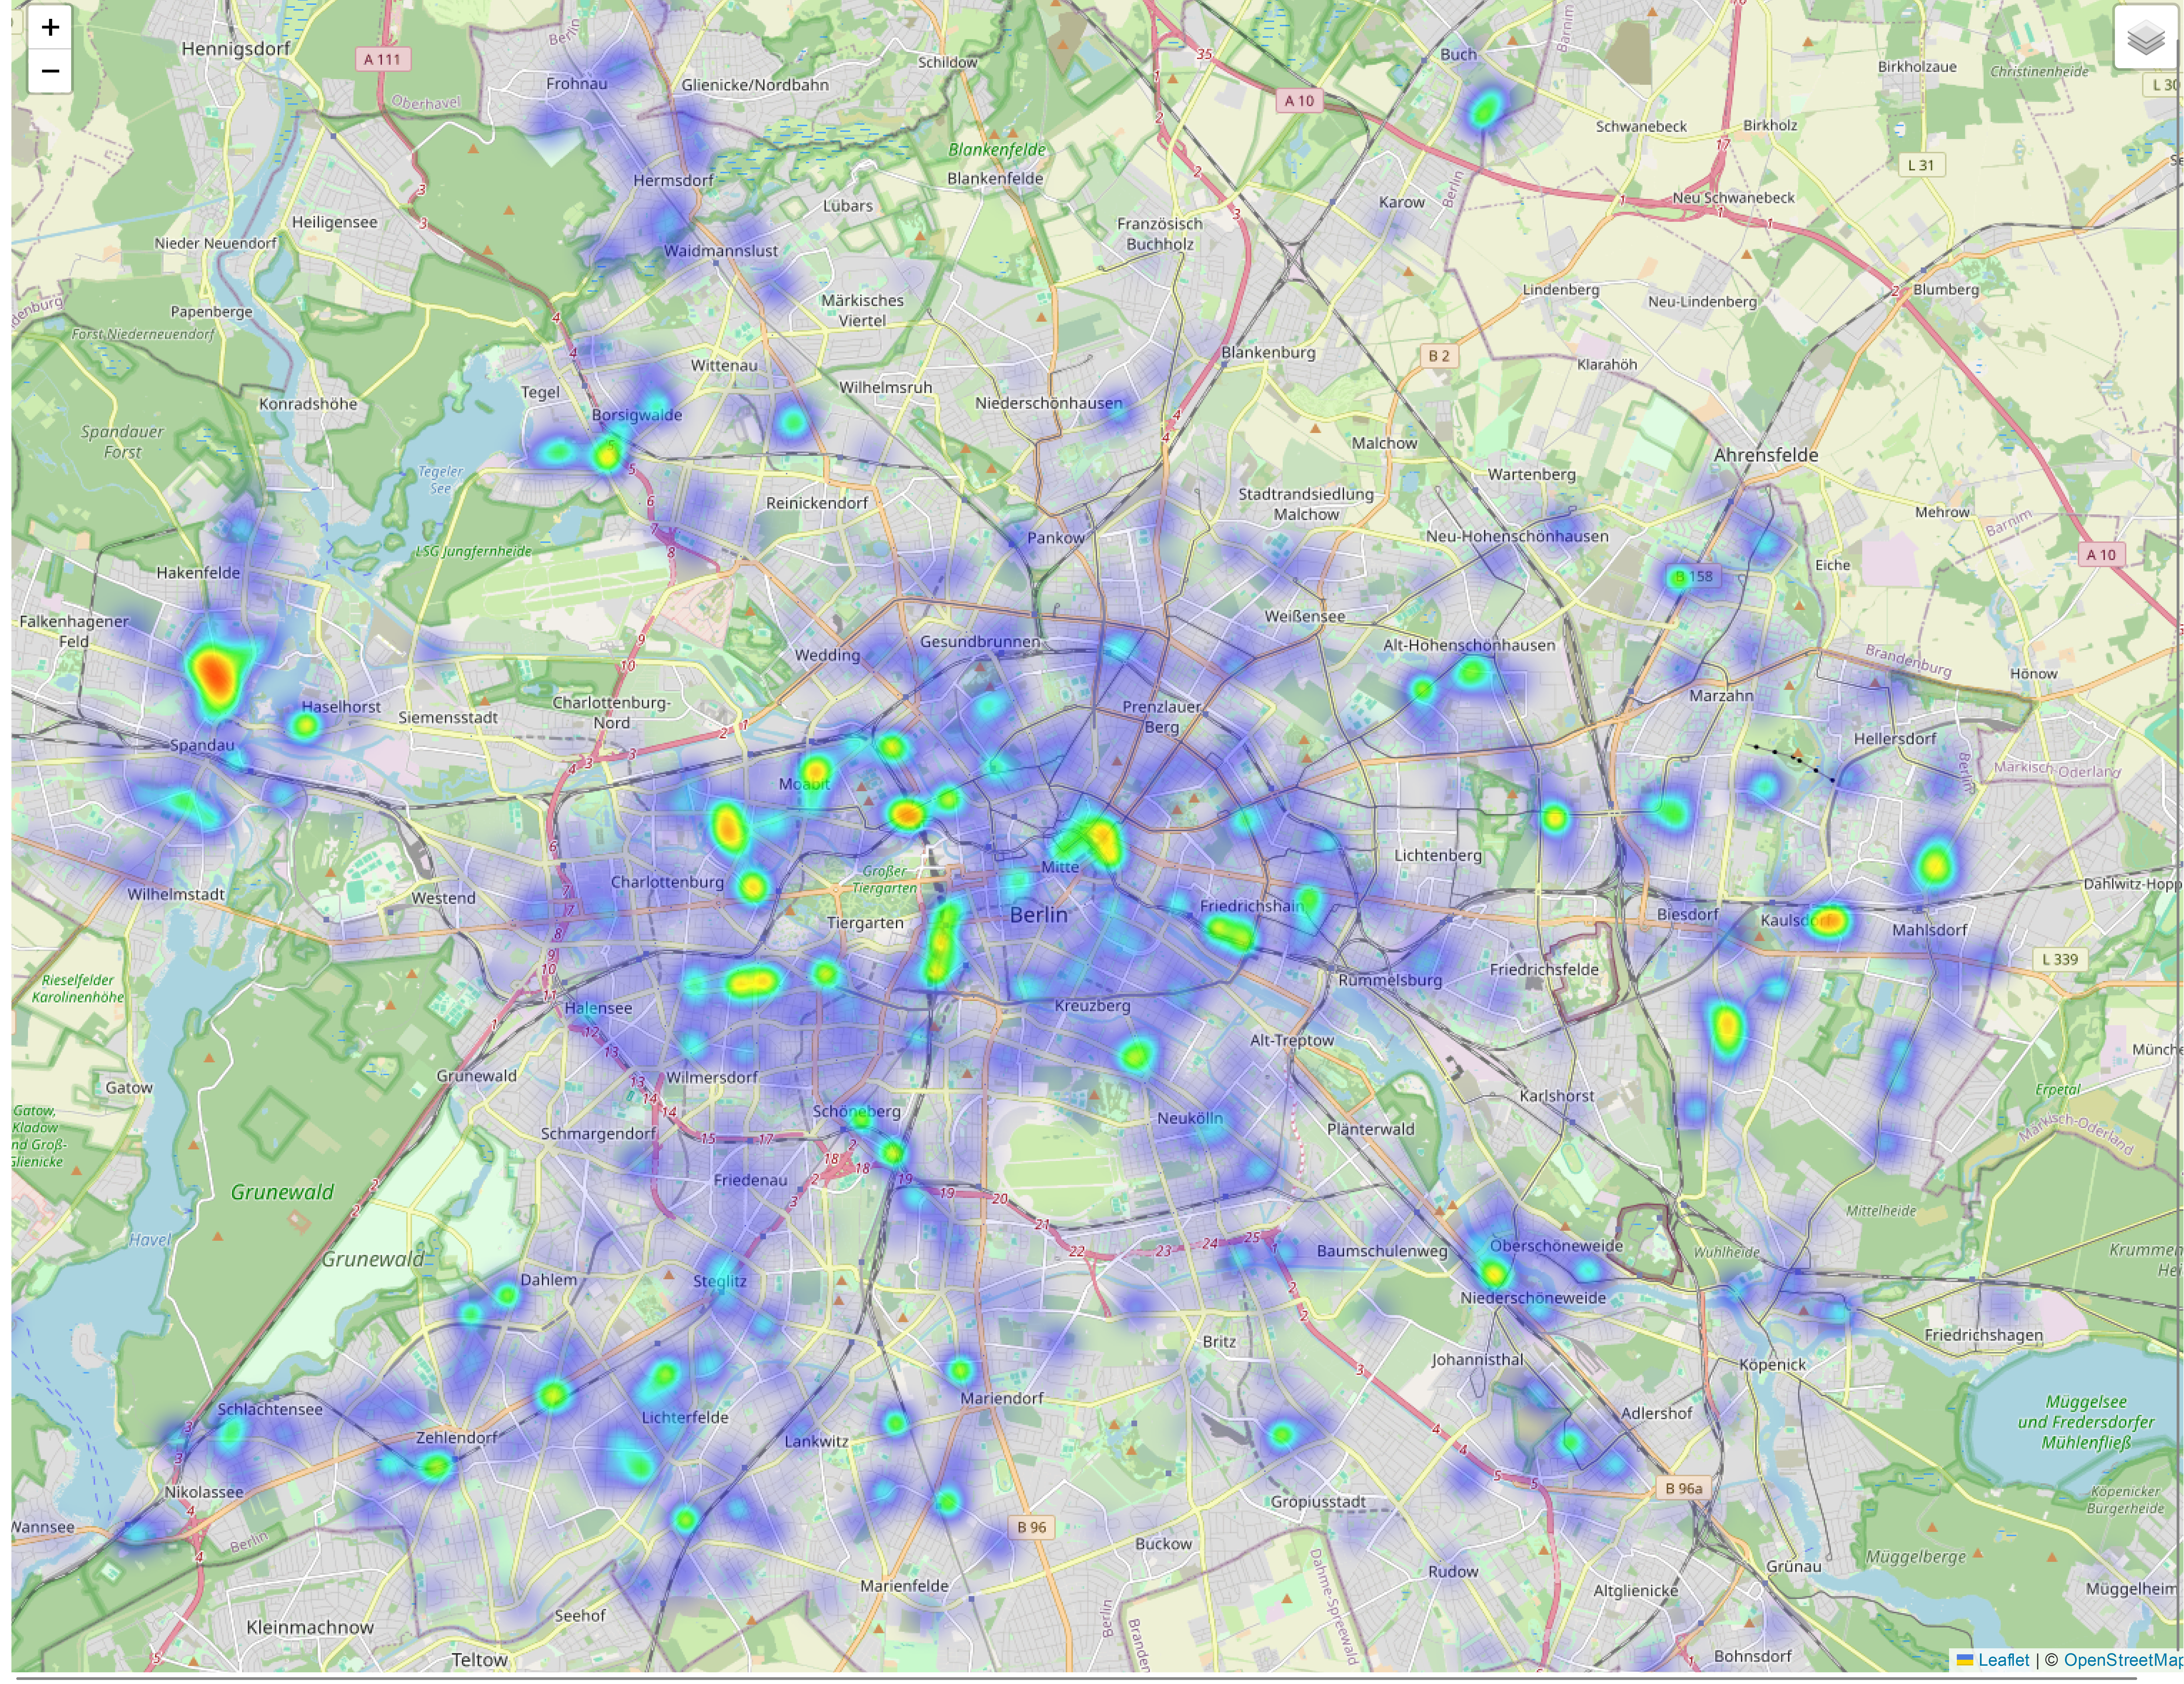
\includegraphics[width=0.75\textwidth]{Bilder/chargerHeatmap.png}
\caption{EV charger heatmap of Berlin\\
          The colors scale with count and are in the following order: Blue - Green - Yellow - Red}\label{fig:chargerdensity}
\end{center}
\end{figure}
\subsection{Adding individual EV charger data}
It could also serve useful to add EV charger locations themselves with their data to confirm that the heatmap is correctly generated and is in accordance with the data. This can be accomplished by creating \verb|L.marker| objects and using \verb|.bindPopup| method to bind a mark-up text to be displayed when an EV charger is clicked on. It is also possible to add a custom icon to the EV charger markers with the \verb|L.icon| function. \\
However as there are 2439 EV chargers in the dataset, the performance becomes a concern with these markers. To alleviate the performance problem, the \verb|Leaflet.markercluster|\cite{markeclusterdocs} plugin can be added via CDN. When markers are added to the \verb|markercluster| created by \verb|L.markerClusterGroup|, the markers that are close together are combined to a single marker, resulting in improved performance. The hidden markers can be revealed by zooming in or clicking on the group marker.\\
\begin{figure}[hbt!]
\begin{center}
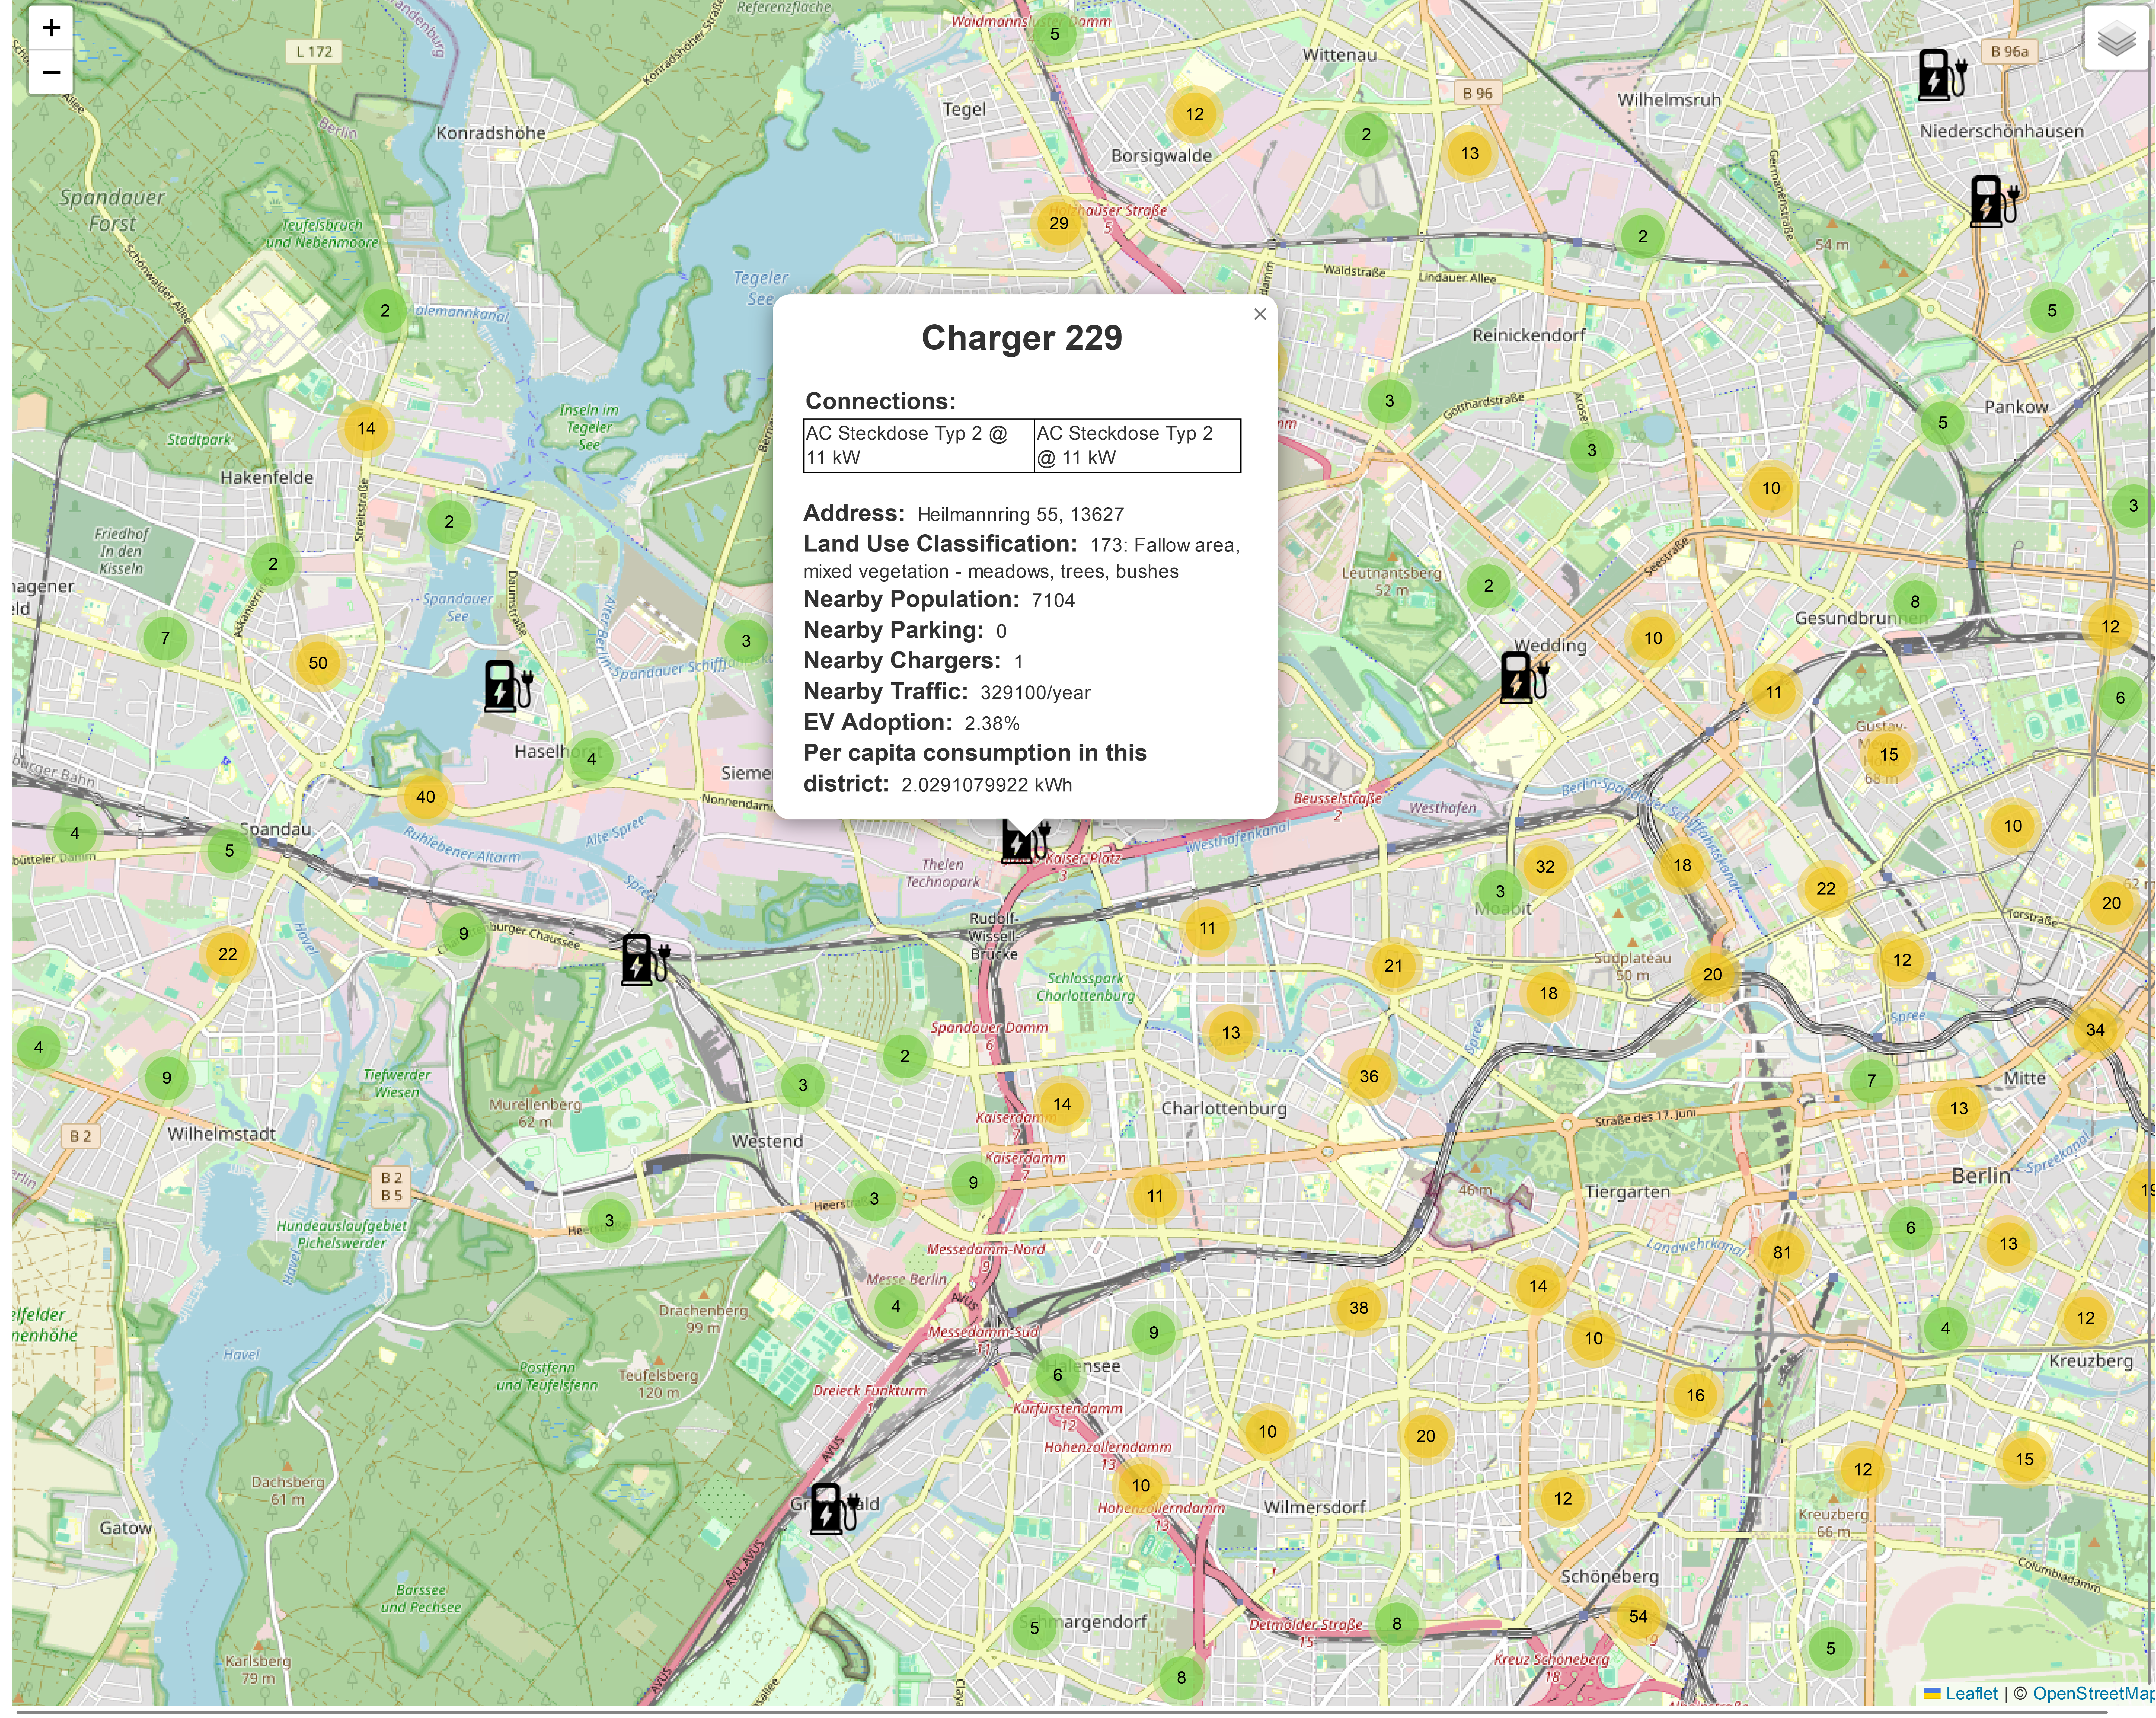
\includegraphics[width=0.75\textwidth]{Bilder/chargermarker.png}
\caption{Single and grouped charger markers with custom popup}\label{fig:chargermarker}
\end{center}
\end{figure}
\section{Methodology}
\subsection{AI Methodologies}
Machine learning and deep learning, which is a subset of machine learning, have been proven to be efficient in finding correlations between large data points. By objectively assigning weights to variables, the high-dimensional task of finding a function to predict optimal EV charger locations can be carried out by many members of the machine learning toolchain.\cite{deploymentproblem} In this section, which AI models are applicable for the task at hand will be explored.
\subsubsection{Supervised Learning}
Supervised learning is a type of learning paradigm that is trained on labeled data. This means that the training set includes both input features and output values. The goal is to find a function that maps the input to the output by adjusting weights of the input features in a linear equation in an iterative process using techniques like gradient descent.\\
The biggest component of supervised learning is also its biggest drawback: the requirement for large amounts of labeled data. With a small dataset, a supervised learning model can over-fit the data, meaning that it can memorize the data set rather than recognize underlying patterns. In real life scenarios, this can be quite time-consuming or expensive.\\
Combined with neural networks, which will be explained later, more complex tasks can be tackled, making supervised learning the best candidate for predicting optimal locations of EV chargers. The exact approach on how to train a supervised learning neural network will be detailed in Section \ref{sec:52}.
\subsubsection{Unsupervised Learning}\label{sec:ulearingexp}
Unsupervised learning is a type of machine learning in which the model is trained on unlabeled data. The model must find patterns and structure on its own to gain insight and make predictions. Unsupervised learning is also used in marketing, anomaly detection and image processing.\\
There are many unsupervised learning techniques, and among the most common is clustering. Clustering tries to group the data points together into clusters. The model trained by unsupervised training can then predict which clusters the new data points belong to. Then it is potentially possible to use a multiple-criteria decision analysis to rank the clusters, reducing the human involvement in the decision making immensely.\\
Unsupervised learning does not have the precision supervised learning has and therefore it is difficult to assess how well the model is performing. Additionally, the patterns that a unsupervised learning model finds might be superficial and may not necessarily represent a real world correlation.
\subsubsection{Reinforcement Learning}
Reinforcement learning is a type of machine learning where a model(agent) interacts and makes decisions about data to achieve a goal. The agent receives rewards and punishments for its decisions based on how wrong the decision was. It is inspired by how humans and animals learn by trial and error.\\
Though it's possible to have the agent go through the trial and error by simulating the environment, the simulation is out of scope for this paper. This approach is more efficient for the modelable problems in the EV landscape. 
\subsubsection{Conclusion}
In section \ref{sec:41} the degree of optimality of an EV charger was squeezed down to single numerical value. And that value is in a spectrum, namely between 0 and 1. Supervised learning algorithms are the best option for linear regression, which is predicting continuous, non-binary outcomes.\\
A machine learning architecture will be proposed using supervised learning and neural networks. However, as explained in section \ref{sec:43}, all available charger utilization datasets are either anonymized(location unknown) or not publicly available. Therefore a real example is unable to be demonstrated. The details of training a model will instead be explained in section \ref{sec:542} for an unsupervised learning model.


\subsection{Neural Network to Predict Efficiency}\label{sec:52}
\subsubsection{How a Neural Network Works}\label{sec:521}
A neural network is a type of learning structure that is inspired by the human brain. A neural network consists of interconnected neurons that alter and pass on information. Neural networks can handle complex tasks compared to other methods and neural networks are the backbone of deep learning.\\
\begin{figure}[hbt!]
\begin{center}
\includegraphics[width=0.75\textwidth]{Bilder/Neural-Networks-Architecture.png}
\caption{ Structure of a neural network\cite{gfgneural}}\label{fig:neural}
\end{center}
\end{figure}\\
A neural network is made up of 5 components:
\begin{enumerate}
    \item \textbf{Neurons:} Each neuron recieves an input, alters it and then passes the value onto the next neuron. All neurons in a layer are connected to all neurons in the previous and the next layer.
    \item \textbf{Layers:} A layer is a group of neurons. A network has input, output and hidden layers. More hidden layers contribute to better accuracy but gives back diminishing returns at the cost of performance.
    \item \textbf{Weights:} A neuron's each connection has its own weight which the value in the neuron is multiplied by.
    \item \textbf{Bias:} Each neuron has a bias term that is added to the value in the neuron
    \item \textbf{Activation function:} Weighted sums are then put through activation functions to introduce non-linearity. Most common examples of activation functions are Rectified Linear Unit(ReLU) and sigmoid functions.
\end{enumerate}
Neural networks are trained in 3 steps:
\begin{enumerate}
    \item \textbf{Forward Propagation:} Input data is passed onto the input layer and then forward through the hidden layers.
    \item \textbf{Loss Function:} The model's prediction is compared to the actual result using a loss function(like Mean Square Error, Binary Cross-Entropy etc.), which measures the error between the predicted output and the expected output.
    \item \textbf{Backpropagation:} The network adjusts the weights and biases using an optimization algorithm to minimize the error.
\end{enumerate}
Neural networks are an excellent choice for handling high dimensional data like all the features of an EV charger location and learning non linear relationships.
\subsubsection{Neural Network Architecture Proposal}\label{sec:proposal}
\begin{figure}[H]
\begin{center}
\includegraphics[width=0.75\textwidth]{Bilder/sdfgsgdfg.png}
\caption{ Neural Network Architecture Proposal}\label{fig:neuraldraft}
\end{center}
\end{figure}
In this model, the EV charger data will be fed to input neurons. It is important here to recognize that though the land use classification is represented by a numerical value, it is a categorical value in actuality. The model should not treat it as a number and as such, should not perform mathematical calculations on it because, for example, adding the category "Housing Area" to "Industrial Area" is not possible. One of the most common ways to circumvent this is using One-Hot Encoding. One-Hot Encoding turns categorical data into a binary vector. In programming languages this is represented by an array like \verb|[1, 0, 0]|. The position of 1 determines the category. This achieves many things. Firstly, now the data has no implicit ordering, meaning that they have no numerical relationship and are independent from each other. Secondly, the encoded data is equidistant and has no ranking or hierarchy. These achieve individuality in data and the model no longer assumes relationships between categories.\\
After the input data is propagated, they arrive in the hidden layers. For the purposes of predicting it is sensible to use 2-4 hidden layers with 64-128 neurons each with \gls{ReLU} activation function to strike a balance between learning prowess and computational overhead.\\
On the output layer there will be a single neuron which holds the predicted efficiency score. Sigmoid can be used for activation function because of its suitability for regression of bounded values.
\begin{figure}[H]
\begin{center}
\includesvg[width=0.75\textwidth]{Bilder/Logisticcurve.svg}
\caption{Sigmoid function\cite{wikisigmoid}}\label{fig:sigmoid}
\end{center}
\end{figure}
For the loss function, mean squared error is more suitable for regression. Although not mentioned in section \ref{sec:521} as a necessary part of a neural network, the Adam(Adaptive Moment Estimation) optimizer can be used as the optimization method. The Adam optimizer is an algorithm commonly used for updating weights and biases during training. In the end the trained model will be able to take in new data and output a prediction based on the training data.\\
All of the necessary tools are present in various libraries for programming languages. These tools remove a lot of development burden and enable training a model with relatively few lines of code. 

\subsection{Grid Partition Method for Results}\label{sec:gridmethod}
Grid partition method refers to the process of dividing a geographical area into smaller, separate grid cells. To figure out which parts of a geographical area(Berlin in the case of this paper) are more suited for deploying EV chargers, a trained model can be used to evaluate each grid cell. The result of the evaluation would be the predicted efficiency score an EV charger placed in the center of that grid would have. Logically, a more divided grid results in more granular data but the compute times can get overbearing fast. The exact grid partition method used in following sections is as follows:
\begin{enumerate}
    \item Berlin is divided into $n \times n$ squares. The grids' center coordinates are saved.
    \item A function is used to consolidate data within a $500m \times 500m$ square centered around the EV charger candidate location.
    \item The collected data for each grid is fed through the trained model and the prediction is saved.
    \item The predictions are scaled into valid ranges and visualized on the map
\end{enumerate}
\iffalse
\begin{figure}[H]
\begin{center}
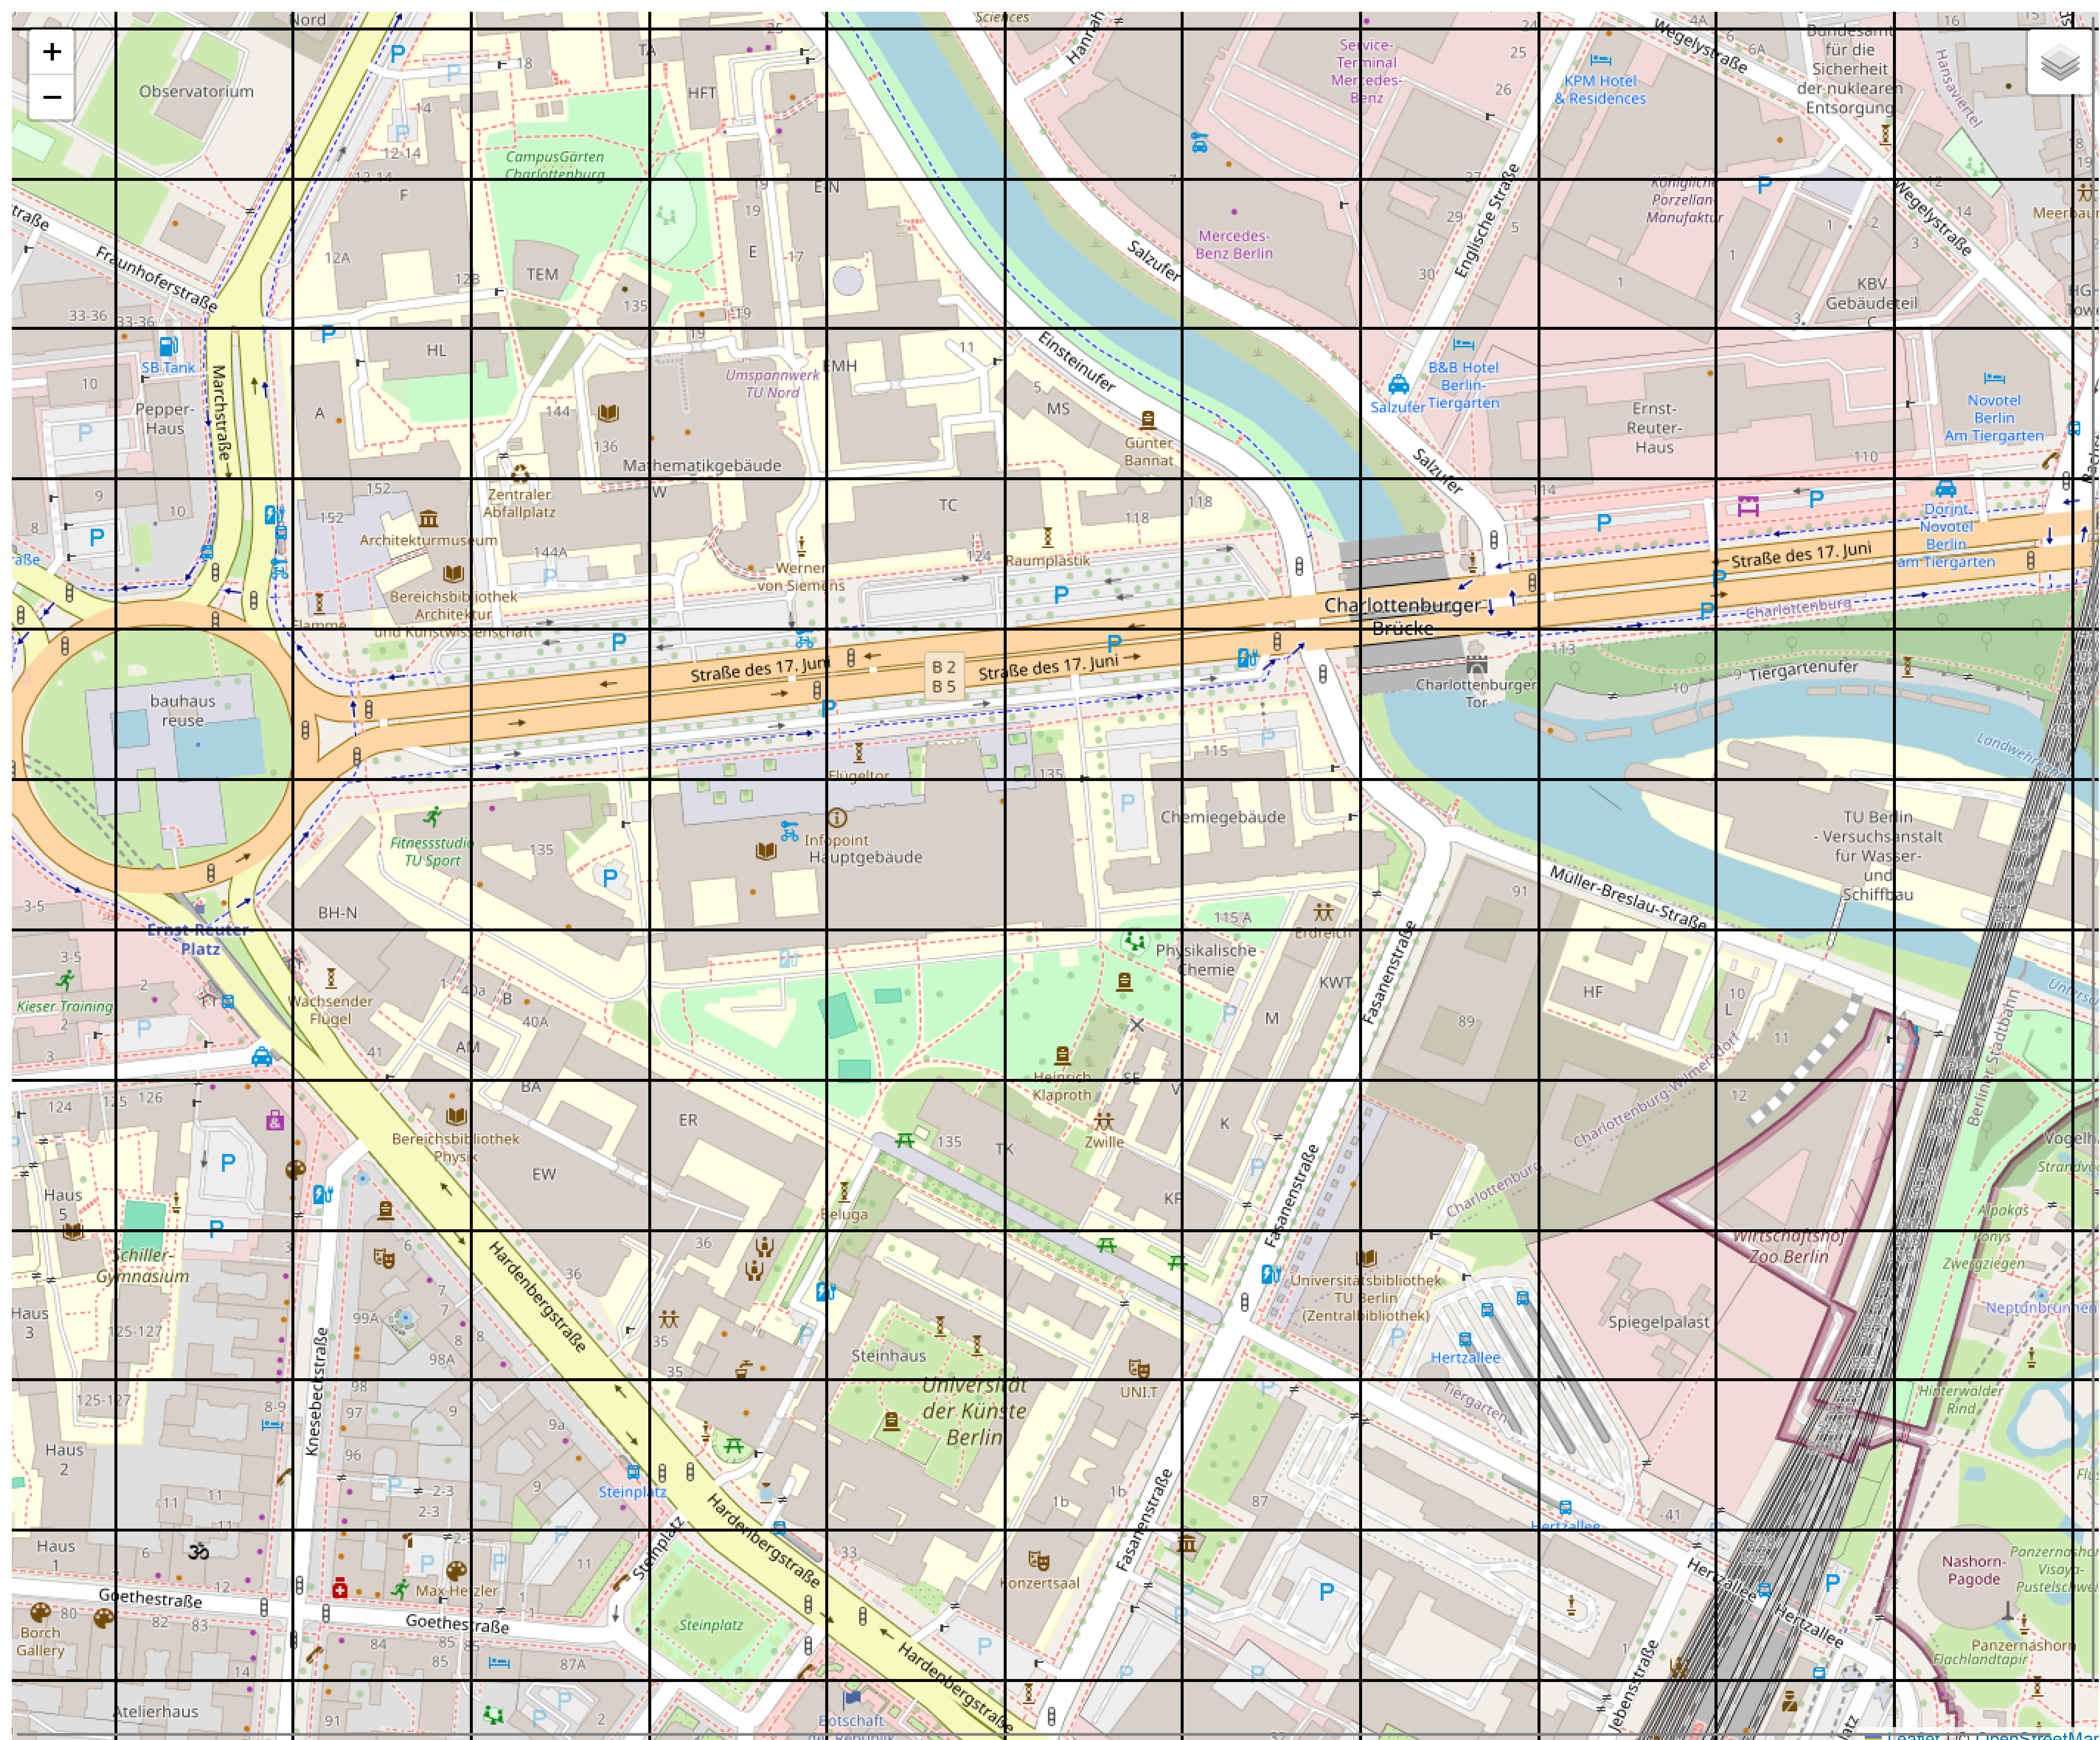
\includegraphics[width=0.75\textwidth]{Bilder/mapgrid.png}
\caption{$500\times500$ grid over Berlin}\label{fig:mapgrid}
\end{center}
\end{figure}
\fi
\subsection{Working with Open Data}
One of the challenges in deploying AI-driven strategies for EV charging station optimization is the absence of publicly available data on charger utilization. This limitation necessitates leveraging alternative methodology and open data sources to approximate demand and make informed deployment decisions. Open data — ranging from traffic and population density to existing charging infrastructure and points of interest—offers a valuable foundation for analysis. With these datasets, it is still possible to generate meaningful insights despite the gaps in charger-specific data. This section explores methods for processing open data to support model development in the context of EV infrastructure planning.
\subsubsection{Using A Pre-Trained Model to Predict Demand}
One of the ways of working around missing data is synthesizing the data. Using a pre-trained model developed by Jayanath et al.\cite{Jayanath2024} it is possible to generate general information about charging events of an EV charger using surrounding area information.\\
Jayanath et al. collected information about a network of 12 direct current fast charging(DCFC) sites in the province of Nova Scotia in Canada. They then trained a supervised learning model to map 4 data sets to charger utilization data. This charger utilization data is also not publicly available.\\
The data points used by Jayanath et al. were:
\begin{itemize}
    \item Traffic volume: Average daily traffic(passing vehicle) count scaled down by a factor of 1000
    \item Local population: Nearby population scaled down by a factor of 1000
    \item Interprovincal highway: This feature is special to Canada and its geography and city design. A city like Berlin is more interconnected thus when considering inside areas of Berlin, interprovincal highways have much less weight in the matter of charger utilization.
    \item Competition defined as:
    \[
        Comp = \frac{\sum^N_{n=1} (P_{kW_n}) \times (25 - Dist_{minutes})^2 \times PlugFactor_n}{P_{kW_{here}} \times 25^2}
    \]
    \begin{itemize}
        \item $P_{kW}$ denotes the total wattage of a charger
        \item $Dist_{minutes}$ denotes the distance to competing charger in minutes. Because finding out the distance in minute requires interacting with an external application programming interface(API), here distance in kilometers were preferred. As the target, 1km was set.
        \item $PlugFactor$ denotes what fraction of EV fleet the \gls{DCFC} charger can serve if it has a proprietary connector that is not compatible with all EVs. This information is not available for Berlin.
    \end{itemize}
\end{itemize}
One concern around using this model is the gaps in data. Therefore this model should and will only be used to enable making more informed decisions when utilization data is absent. The results should be seen as relative or some sort of ranking between EV chargers.\\
Jayanath et al. trained a regression model using these data points and published the regression coefficients. The results are as follows:
\begin{table}[!h]
\begin{center}
\begin{tabular}{ | c | c | c | c | c | }
\hline
 Variable & Units & Lower a & Best a & Upper a \\ 
 \hline
 Traffic, $a_1$ & $Events/10^3\cdot ADT$ & 17 & 35 & 53 \\
 \hline
 Population, $a_2$ & $Events/kPop$ & -23 & 8 & 39 \\
 \hline
 Competition, $a_3$ & $Events/Comp$ & -152 & -77 & -2 \\
 \hline
 InterProv, $a_4$& $Events/InterProv$ & 980 & 1335 & 1690 \\
 \hline
\end{tabular}
\caption{ Regression coefficients for each of the four geographic explanatory variables, with 95th percent confidence interval coefficients, Jayanath et al.\cite{Jayanath2024} }
\end{center}
\end{table}

The predicted number of daily charging events per year can be expressed as:
\[
Pred_i = a_21 \times Traf_i + a_2 \times Pop_i + a_3 \times Comp_i + a4 \times InterProv_i
\]
After normalizing the data and using a similar function to the the efficiency score function in section \ref{sec:41}, the vacancy heatmap of EV chargers in Berlin can be generated. 
\begin{figure}[H]
\begin{center}
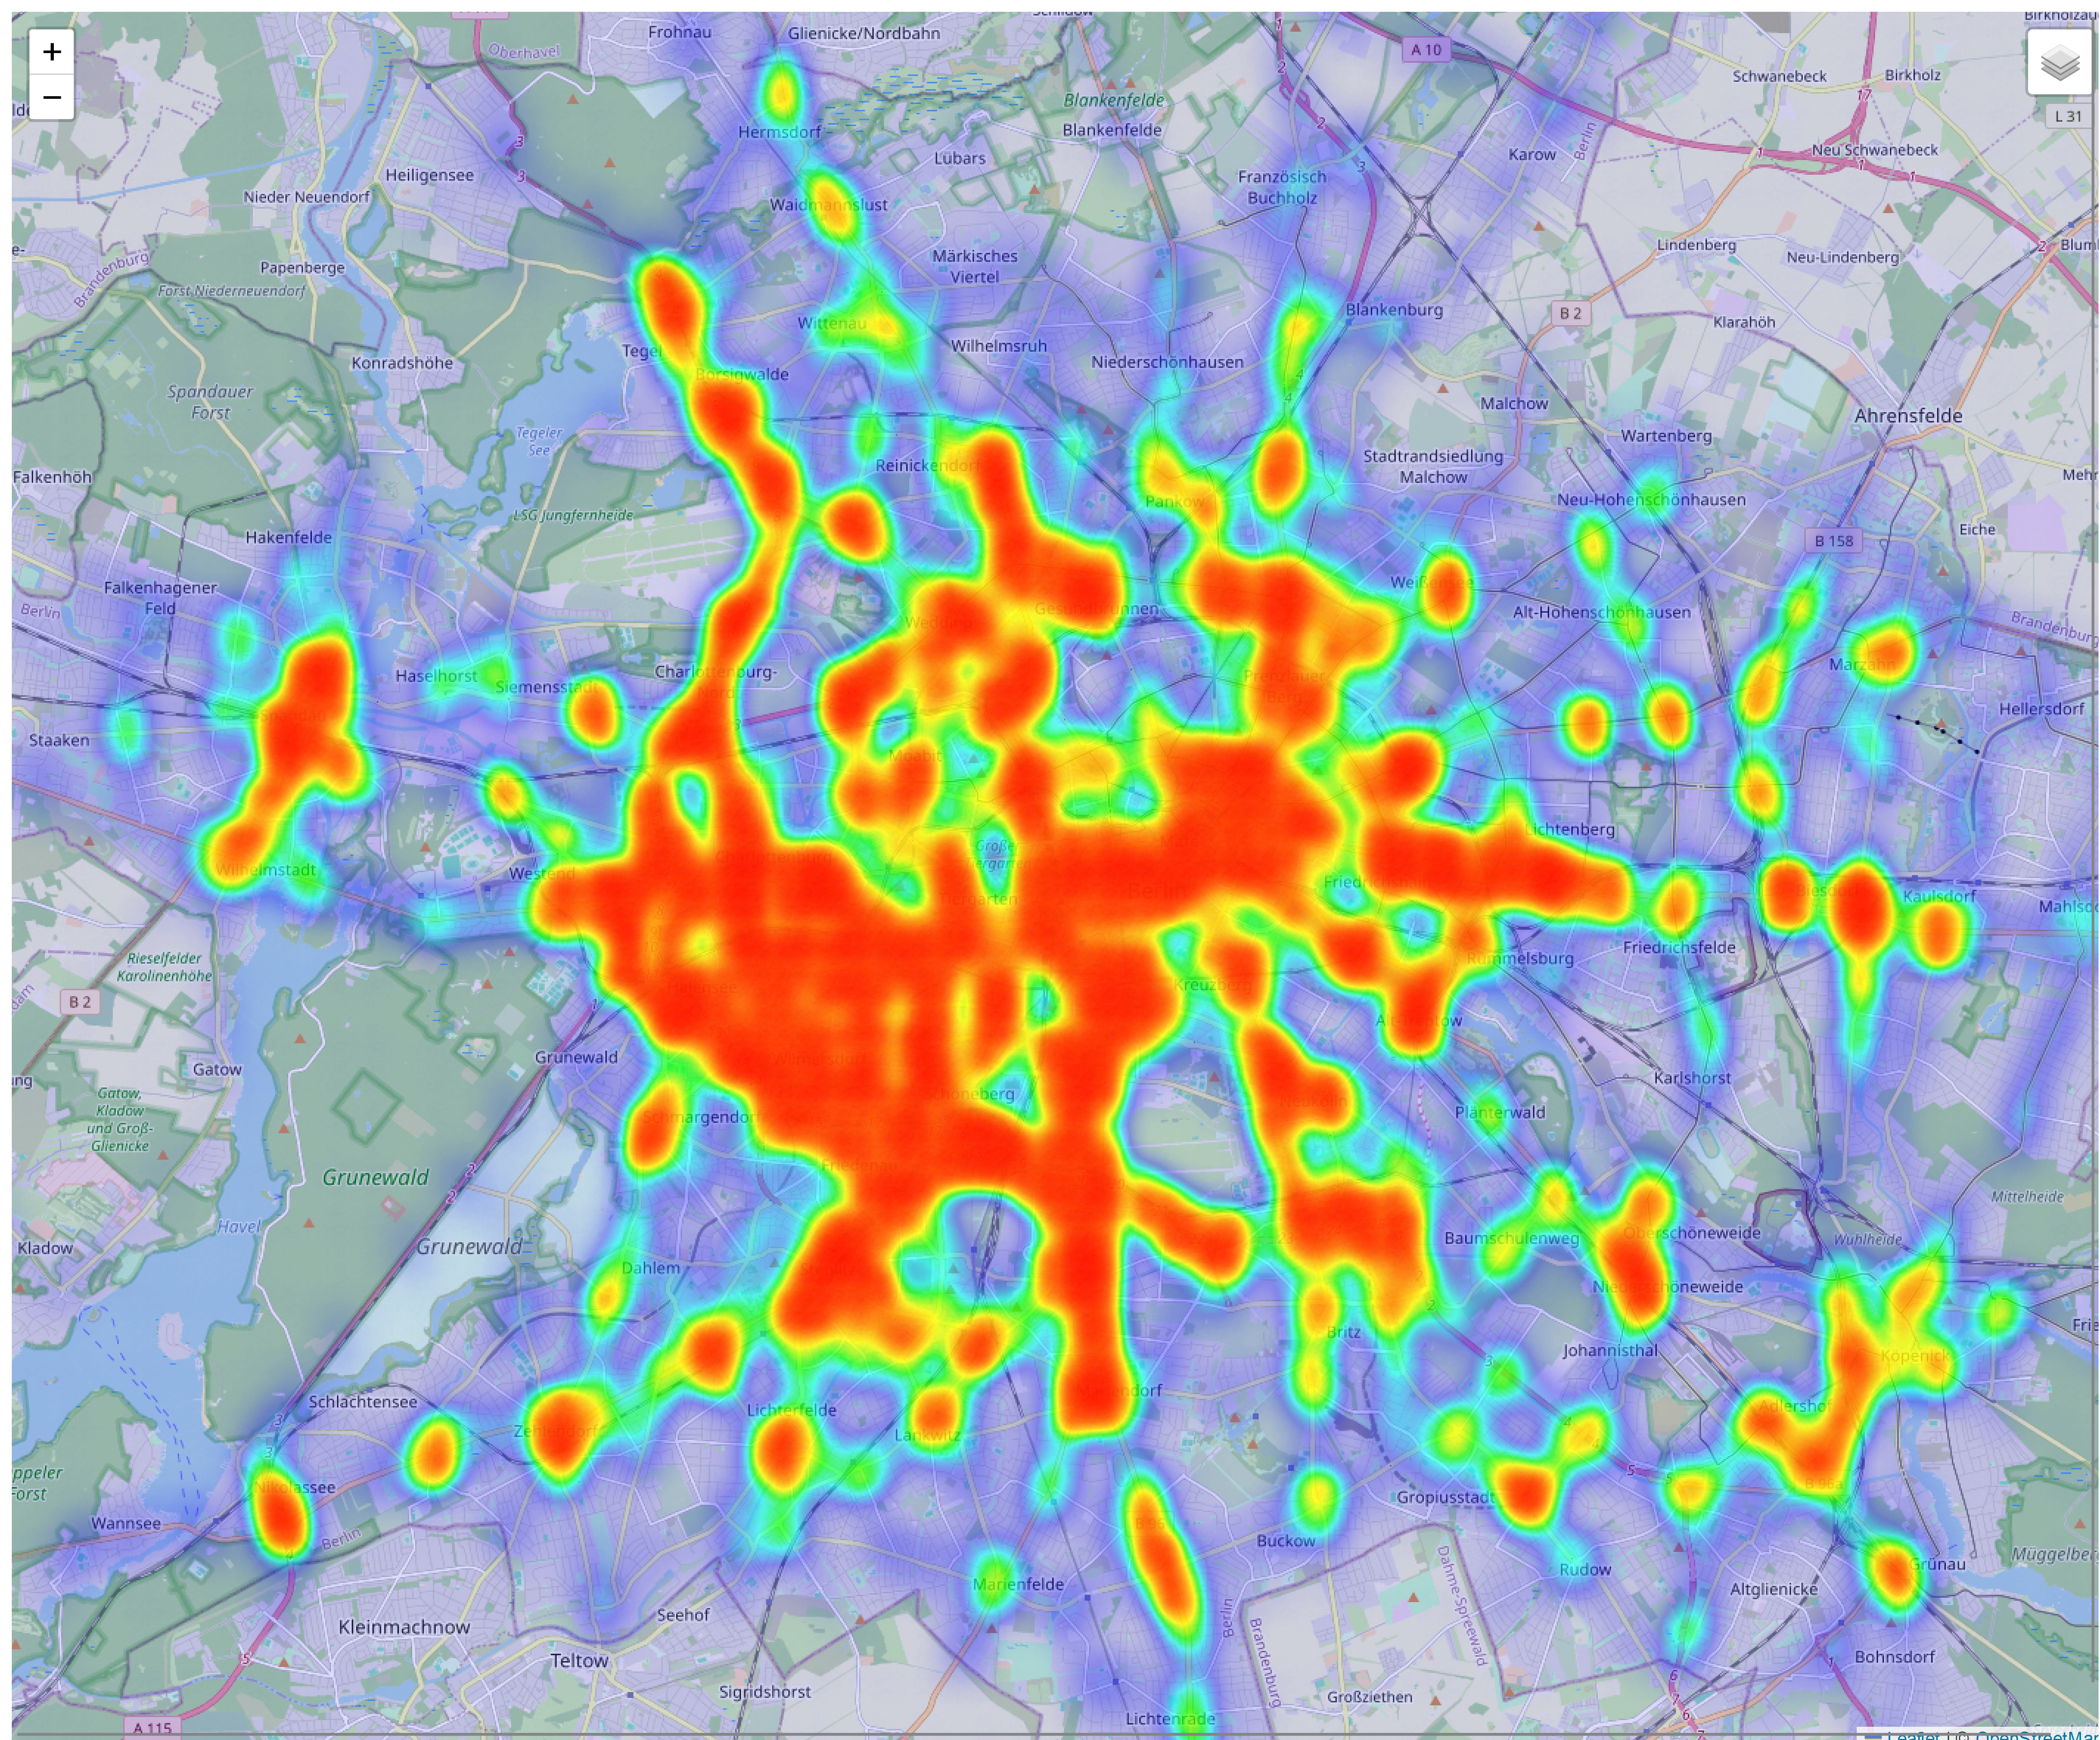
\includegraphics[width=0.75\textwidth]{Bilder/jayanath.png}
\caption{ Heatmap of Berlin using the regression model by Jayanath et al.\cite{Jayanath2024} and scoring.\\
          The colors scale with score and are in the following order: Blue - Green - Yellow - Red}
\end{center}
\end{figure}
Note that this map doesn't show absolute efficiency but rather it highlights EV chargers that lie around 50th percentile of predicted yearly charging events.\\
From the regression coefficients it is abundantly clear that Jayanath et al.'s model is highly biased towards traffic hotspots and the map reflects this tendency. Such skewed performance can lead to unintended consequences, including the misallocation of resources or inaccurate predictions in areas with lower traffic density. For instance, the model may overestimate traffic congestion in peripheral areas or fail to identify emerging congestion patterns. Addressing this issue would entail a more dimensional model that is trained with more diverse data such as the one proposed in section \ref{sec:proposal}.


\subsubsection{Unsupervised Learning}\label{sec:542}
An unsupervised learning model is the model that can provide most insight with the available, unlabeled data. This section focuses on the steps that were taken to train an unsupervised learning model from the ground up using publicly available data for Berlin. The model was coded with the Python programming language and the packages used were \verb|yellowbrick, scikit-learn| and \verb|matplotlib|. \\
Machine learning models work best with data that lies within the same numerical range. One data point ranging in a disproportionately bigger spectrum can cause learning errors as the data point with bigger values would have a bigger impact on the regression equation. Therefore it is of immense importance to fit all the data points into the same range. This can be achieved with the following code:
\begin{minted}[frame=lines, framesep=2mm, baselinestretch=1.2, fontsize=\footnotesize, linenos]{python}
    from sklearn.preprocessing import MinMaxScaler
    
    scaler = MinMaxScaler((0, 1))
    scaled_data = scaler.fit_transform(data)
\end{minted}
First a \verb|MinMaxScaler| object was initialized with tuple of the preferred range of 0 to 1. Then the \verb|fit_transform| method was used to scale the data from 0 to 1. With the data properly scaled, building the model can commence.\\
For the unsupervised learning technique, clustering explained in section \ref{sec:ulearingexp} was chosen. As for the clustering method, the K-Means method was chosen for its simplicity and and faster performance. The K-Means method however requires predetermining how many clusters there should be. To help with this decision, the "elbow" method is the most commonly used\cite{KFG}. The elbow method works by calculating the within-cluster sum of squares (WCSS) for each number of clusters k. \gls{WCSS} measures how tightly points are grouped within a cluster, with smaller values indicating better clustering. To figure out the optimal number of clusters for our data, \verb|KElbowVisualizer| module can be used.
\begin{minted}[frame=lines, framesep=2mm, baselinestretch=1.2, fontsize=\footnotesize, linenos]{python}
    from yellowbrick.cluster import KElbowVisualizer
    
    kmeans = KMeans()
    elbow = KElbowVisualizer(kmeans, k=(2, 20))
    elbow.fit(scaled_data)
    elbow.show(block=True)
\end{minted}
Outputs the following graph:
\begin{figure}[H]
\begin{center}
\includesvg[width=0.75\textwidth]{Bilder/savedSVG.svg}
\caption{ Distortion score elbow for K-Means clustering }
\end{center}
\end{figure}
Elements of the graph are:
\begin{enumerate}
    \item \textbf{Distortion score} which is depicted as the y-axis on the left. The distortion score is the WCSS.
    \item \textbf{Fit time} which is depicted as the y-axis on the right(in seconds). The fit time is how much time it takes for the model to learn the data.
    \item \textbf{Number of clusters($k$)} which is the x-axis
    \item \textbf{Blue line} which is distortion score versus number of clusters
    \item \textbf{Green line} which is fit time versus number of clusters
    \item \textbf{Dashed black line} which is the elbow point
\end{enumerate}
The elbow point which lies at $k=7$ for this particular dataset is the point where distortion point stops decreasing significantly as k increases. Adding more clusters beyond this points increases fit time with diminishing returns. Although the fit time suggests that it is less than tenth of a second even for higher clusters number, it is important to set an optimal number of clusters for better scalability without sacrificing accuracy.\\
With the number of clusters determined, the model can be initialized and trained with just 3 lines of code:
\begin{minted}[frame=lines, framesep=2mm, baselinestretch=1.2, fontsize=\footnotesize, linenos]{python}
    from sklearn.cluster import KMeans
    
    kmeans = KMeans(n_clusters=7)
    data['cluster'] = kmeans.fit_predict(scaled_data)
\end{minted}
This code trains the model and adds the cluster information to the data. The criteria for each cluster can be shown with the following code:
\begin{minted}[frame=lines, framesep=2mm, baselinestretch=1.2, fontsize=\footnotesize, linenos]{python}
    data[['anteilelektrogesamt','traffic_near','pop_near','charger_near', 
    'park_near', 'class','cluster']]\
    .groupby('cluster')\
    .agg({'max', 'min'})
\end{minted}
This outputs the following table:
\begin{table}[!h]
\hskip -1.1cm
\begin{tabular}{|l|l|l|l|l|l|l|l|l|l}
\toprule
\multicolumn{3}{|c|}{p\_EV} & \multicolumn{3}{|c|}{traffic\_near} & \multicolumn{3}{|c|}{pop\_near} & \multicolumn{1}{r}{...} \\
\midrule
mean & min & max & mean & min & max & mean & min & max & ... \\
\midrule
4,08 & 0,94 & 14,82 & 134.182,72 & 7.900,00 & 403.500,00 & 3.444,92 & 0,00 & 11.629,00 & ...\\
6,38 & 1,64 & 24,33 & 355.282,84 & 23.200,00 & 786.450,00 & 10.721,11 & 1.088,00 & 17.295,75 & ...\\
16,11 & 5,24 & 24,33 & 662.738,67 & 332.400,00 & 786.450,00 & 4.122,35 & 85,00 & 11.640,00 & ...\\
4,78 & 0,94 & 17,67 & 213.193,26 & 6.400,00 & 664.700,00 & 3.950,57 & 0,00 & 16.416,00 & ...\\
12,75 & 1,94 & 21,00 & 364.321,37 & 164.900,00 & 786.450,00 & 8.095,70 & 1.760,00 & 12.754,00 & ...\\
4,50 & 1,35 & 21,00 & 458.312,69 & 167.100,00 & 786.450,00 & 7.411,93 & 6,00 & 16.620,00 & ...\\
4,34 & 1,94 & 14,41 & 169.064,54 & 11.000,00 & 514.600,00 & 3.601,63 & 19,00 & 11.033,00 & ...\\
\bottomrule
\end{tabular}
\caption{ Criteria for clusters 0-6(truncated). }
\end{table}\\
Any EV chargers with data that falls within values of a row gets grouped into its respective cluster.\\
Geographical data is not random; it is inherently structured and influenced by underlying patterns, processes, and relationships. Therefore some clusters are inevitably more populated than others. The distribution of clusters can provide valuable insights into existing infrastructure. Clusters shrink massive raw data into a more digestible size. They also signal which patterns are significant enough for a machine learning algorithm to classify it as a cluster. Now that the model learned from the data and assigned each entry a cluster, the distribution of clusters can be visualized with the following code.
\begin{minted}[frame=lines, framesep=2mm, baselinestretch=1.2, fontsize=\footnotesize, linenos]{python}
    import seaborn as sns

    # Defines the color palette
    pal = ["#682F2F","#B9C0C9", "#9F8A78","#F3AB60"]
    
    # Create the count plot
    pl = sns.countplot(x=combo["cluster"], palette= pal)
    pl.set_title("Distribution Of The Clusters")
    plt.show()
\end{minted}
This outputs the following graph:
\begin{figure}[H]
\begin{center}
\includesvg[width=0.75\textwidth]{Bilder/clusterDistribution.svg}
\caption{ Distortion score elbow for K-Means clustering }
\end{center}
\end{figure}
It is clear from the graph that the distribution is not uniform. This is to be expected from the geographical data of a big area. If a more uniform distribution is desired for more granular information, it can be achieved by doing one or a combination of the following:
\begin{itemize}
    \item Using a smaller area
    \item Using stricter outlier detection
    \item Increasing the number of clusters
    \item Balancing the data by resampling - Resampling means reducing the number of entries in the dominating data range and/or increasing the number of entries in minority data ranges by duplication or synthesis
    \item Using a different initialization method for K-Means - Can be passed to \verb|KMeans()| function as optional argument to maximize distance between clusters
    \item Splitting the clusters manually post-training
    \item Using an alternate clustering method
\end{itemize}
Now that the training is complete, new data can be passed to the model to predict its cluster using the following code:
\begin{minted}[frame=lines, framesep=2mm, baselinestretch=1.2, fontsize=\footnotesize, linenos]{python}
    # Create a new entry as pandas DataFrame with appropriate columns
    new_entry = pd.DataFrame([[4.07, 12322.0, 7.0, 4540, 5.0, 10]], columns=['p_EV', 'traffic_near', 
    'pop_near', 'charger_near', 'park_near', 'class'])
    
    # Create a scaler and scale the entry
    scaler = MinMaxScaler((0, 1))
    new_entry_scaled = sc.fit_transform(ls)
    
    # Predict the new entry's cluster
    cluster = kmeans.predict(new_entry_scaled)
    display(cluster)
    
    # Output: array([0])
    # This means that the model predicted this new entry to belong to cluster 0
\end{minted}
Splitting Berlin into a $250 \times 250$ grid using the grid partition method explained in section \ref{sec:gridmethod}, which parts fo Berlin belong to which cluster can be determined. To visualize this, each cluster can be associated with a color and put into an $250 \times 250$ image where each pixel represents a cell on the grid using the following code:
\begin{minted}[frame=lines, framesep=2mm, baselinestretch=1.2, fontsize=\footnotesize, linenos]{python}
    from PIL import Image
    # Dictionary that associates a cluster with a color(RGBA values)
    cluster_color = { 0: (199, 44, 72, 120), 1: (123, 104, 238, 120), 2: (49, 145, 119, 120),
    3: (204, 119, 34, 120), 4: (137, 207, 240, 120), 5: (152, 119, 123, 120), 6: (240, 220, 130, 120)}

    # Set pixel values of each cell
    pixels = grid_cells['cluster'].copy(deep=True)
    pixels = pixels.apply(lambda x: cluster_color[x])
    pixels = pixels.to_numpy()

    # Generate and save the image
    img = Image.new('RGBA', (500, 500))
    img.putdata(pixels)
    img.save('path/to/save/to')
\end{minted}
The generated image can then be laid over the Berlin map using the \verb|L.imageOverlay(image|\\ \verb|, [coordinates])| from the \verb|Leaflet.js| library. The resulting image is as follows:
\begin{figure}[H]
\begin{center}
\includegraphics[width=0.75\textwidth]{Bilder/ulearningvis.png}
\caption{ Clusters in Berlin }
\end{center}
\end{figure}
The information these results provide can be taken even further by employing the Analytic Hierarchy Process(AHP). \gls{AHP} is a structured decision-making framework developed by T. Saaty in the 1970s at the Wharton School of the University of Pennsylvania. AHP consist of comparing criteria pairwise and giving them relative values(X is $k$ times more important than Y). These relative values are then combined to assign an absolute weight to all the criteria\cite{AHP}. This breaks complex decisions down into smaller, more manageable components.\\
As an example, the following values were chosen:

\begin{table}[H]
    \centering
    \begin{tabular}{ccccccc}
        &p\_EV &  traffic\_near& charger\_near & pop\_near & park\_near & class\\
        & 1,5 &1,2  & 2 & 1,2 & 1,2&\\
    \end{tabular}
    \caption{Relative importance values. Each value represents how much more important the criterion is than the next criterion}
\end{table}
Extrapolating these values into a square matrix and finding the eigenvector of said matrix gives absolute weights for each criterion. This can be proceeded by multiplying the weights with each cluster's mean or median values to come up with a numerical representation of that cluster's importance\cite{KFG}. After modifying these numbers using a similar function to the the efficiency score function in section \ref{sec:41}, it can be used along with grid data to generate a heatmap.
\iffalse
\begin{table}
    \centering
    \begin{tabular}{|c|c|}
    \hline
        Cluster & AHP Score\\
        \hline
         0& 46352.045787\\
         \hline
         1& 31239.315776\\
         \hline
         2& 49421.305804\\
         \hline
         3& 105251.054142\\
         \hline
         4& 115853.831340\\
         \hline
         5& 80567.358695\\
         \hline
         6& 158067.816601\\
         \hline
    \end{tabular}
    \caption{AHP scores of clusters}
\end{table}
\fi

\begin{figure}[H]
\begin{center}
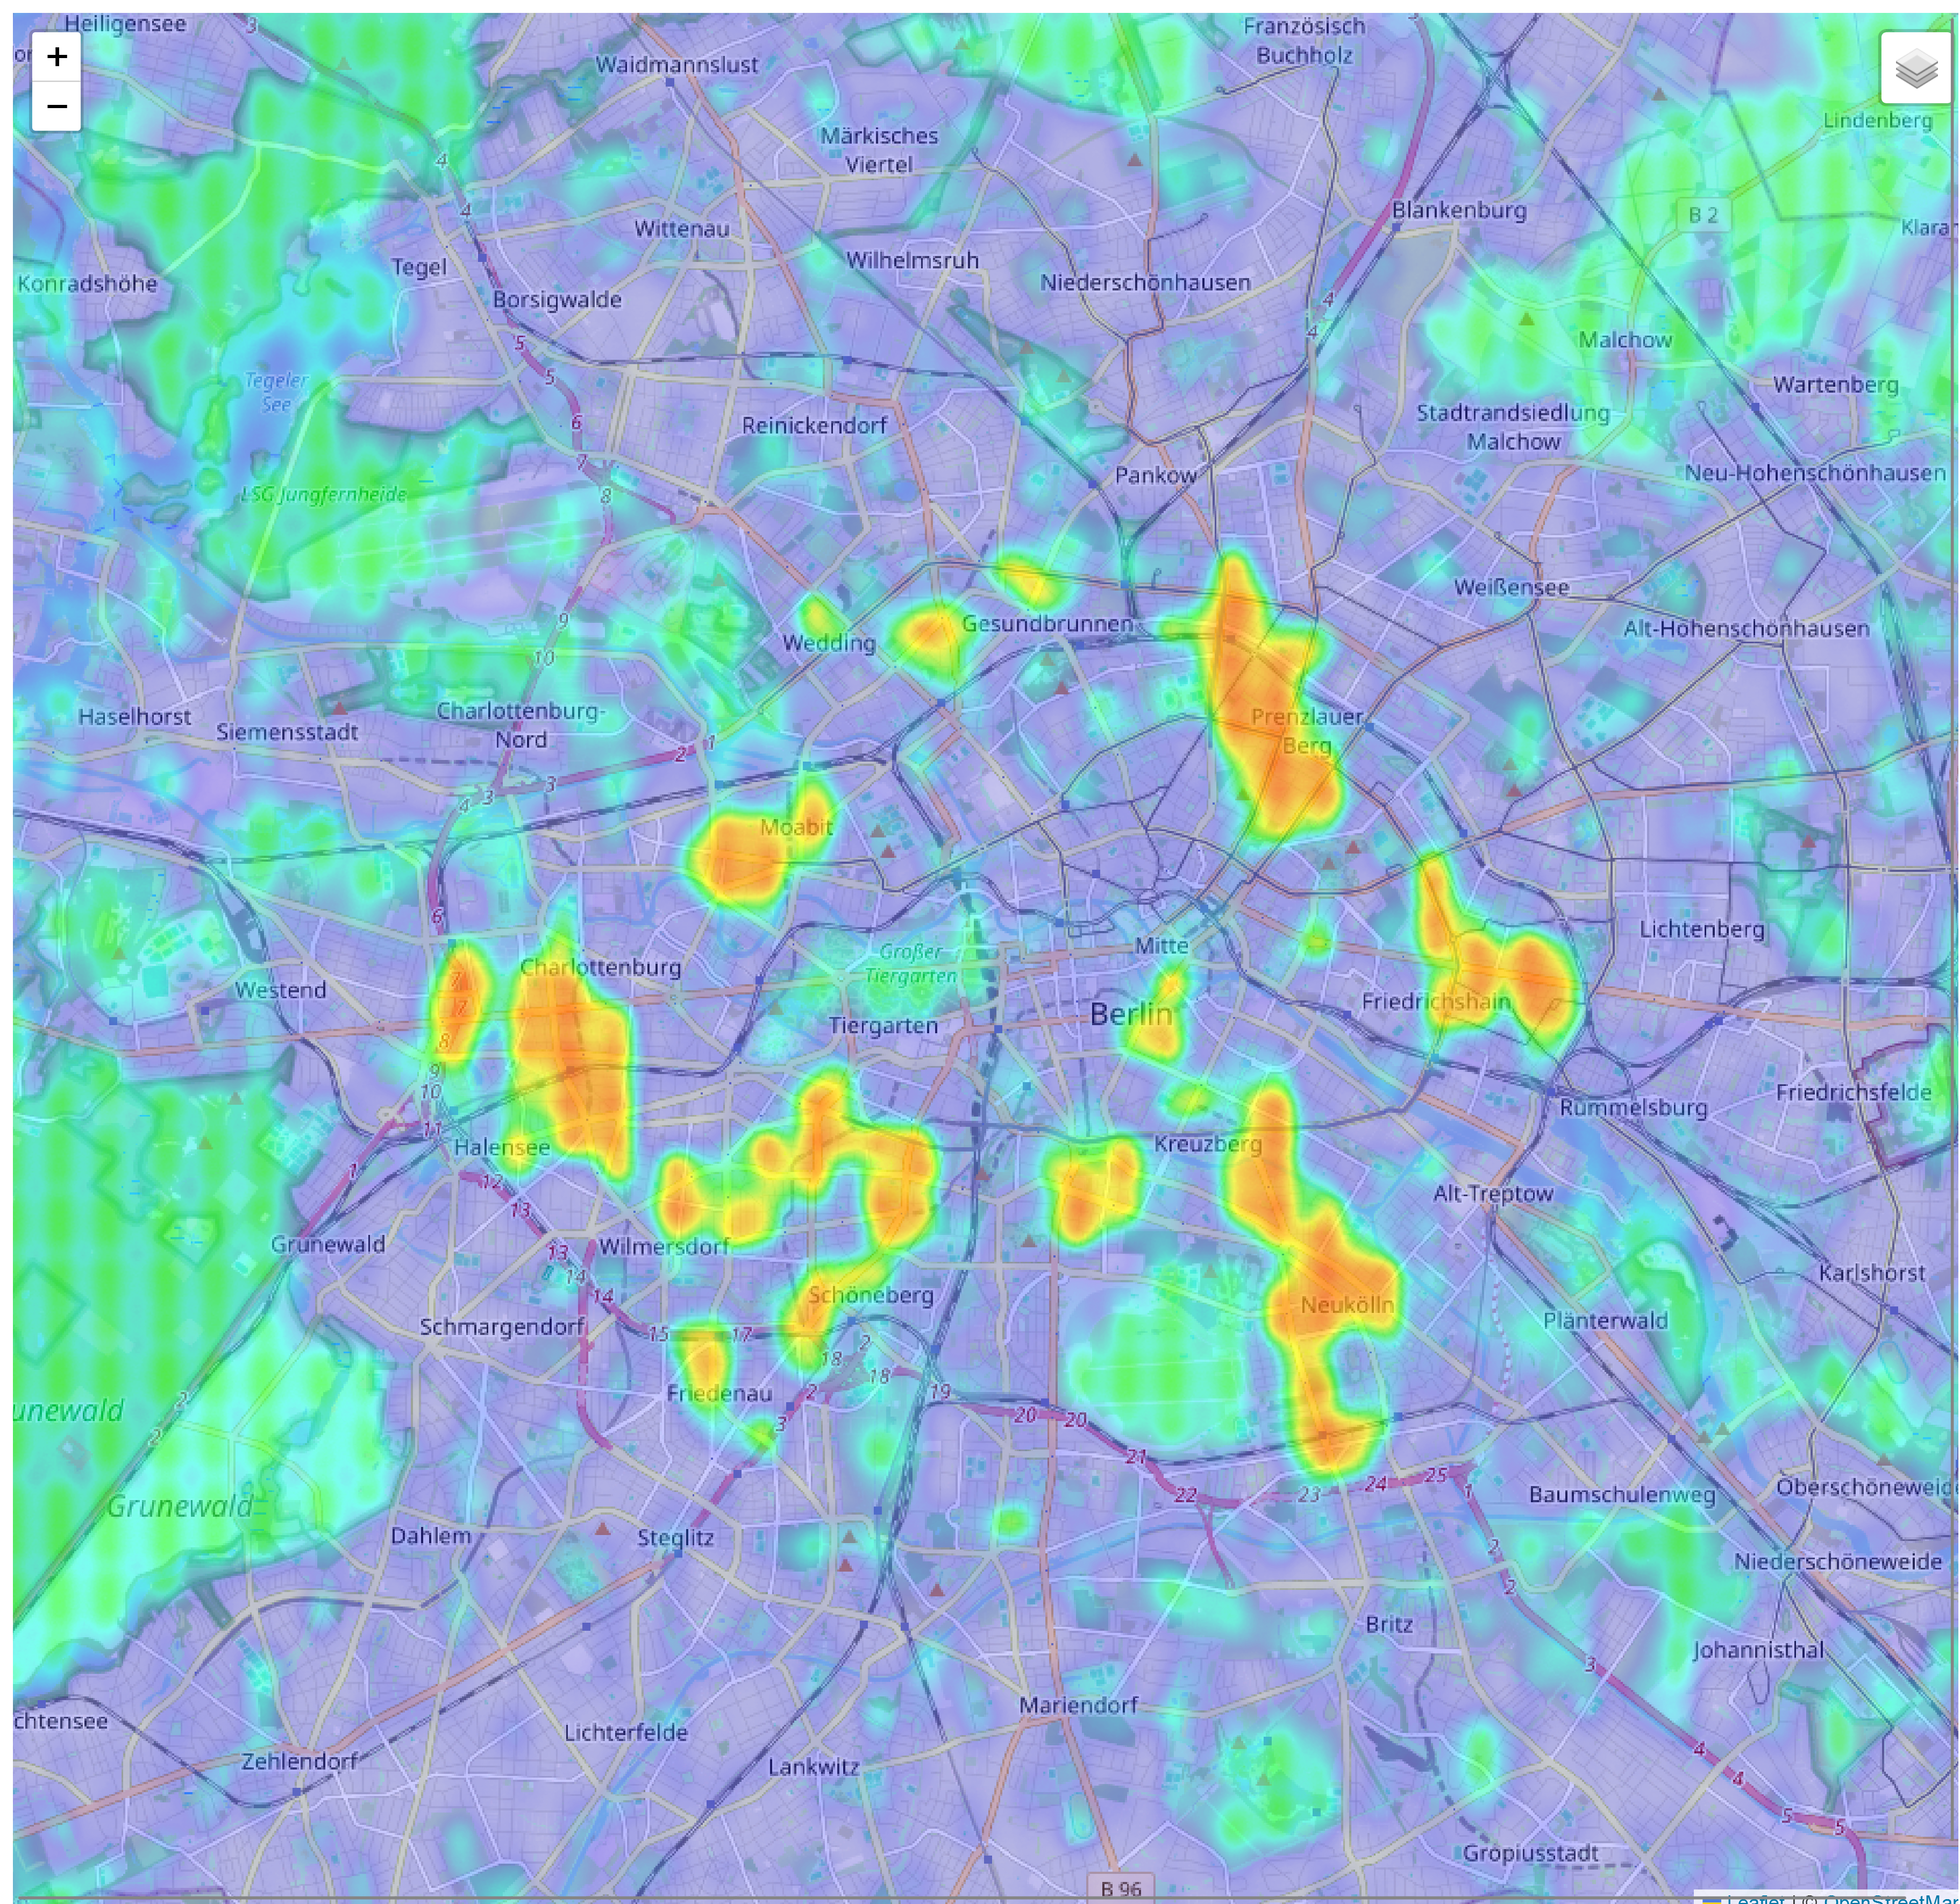
\includegraphics[width=0.75\textwidth]{Bilder/ahpvis.png}
\caption{ Heatmap with modified AHP results \\
          The colors scale with score and are in the following order: Blue - Green - Yellow - Red}
\end{center}
\end{figure} 
This map can be tweaked by tuning the relative weights in the AHP. This aspect makes unsupervised learning using AHP very versatile and able to adapt to new revelations in EV charger data.\\
\iffalse
\section{Planning and Optimization of Electric Vehicle Charging Stations in Berlin: Environmental and Strategic Approaches}
\begin{itemize}
    \item Environmental factors: factors such as rainfall and temperature affect charging station durability and functionality.
    \item CO2 emission distribution: determining where to locate charging stations based on the analysis of high-emission urban areas and low-emission rural areas.
    \item Strategic location: reducing pollution in urban areas and preserving clean air in rural areas by focusing on high-emission areas.
    \item Sustainability in rural areas: protecting low-emission areas and taking measures to achieve this by prioritizing environmentally friendly transportation.
    \item AI-driven optimization: the positioning of stations and efficient use of resources can be adjusted with the help of AI.
    \item Contribution to climate goals: contribute to achieving the environmental sustainability and climate goals targeted for Berlin.
\end{itemize}
These approaches aim to provide effective solutions to the challenges of developing an efficient EV charging station network.

\subsection{Air Quaility}\label{sec:42}

\begin{figure}[H]
\begin{center}
\includegraphics[width=0.75\textwidth]{Bilder/kaan1.png}
\caption{Example of Charging Stations Based on Traffic Flow}\label{fig:kaan1}
\end{center}
\end{figure}



\subsubsection{Pollution Categories in Berlin}\label{sec:43}
Pollution levels in Berlin can be grouped into two categories: 
\begin{itemize}
    \item High Pollution Areas 
    \item Low Pollution Zones
\end{itemize}
\subsubsection{High Pollution Areas:}\label{sec:43}
Pollution levels in Berlin can be grouped into two categories: 
\begin{itemize}
    \item Air pollution is more intense in regions surrounding the city center, such as Spreestinsel.	
    \item PM2.5 and NO2 levels are between 50-55, which shows there is a traffic jam and many fossil fuel vehicles.
    \item Likewise, high pollution values of between 42-48 are detected in the southeast of Berlin.
    \item impacts for children, the elderly, and individuals with respiratory conditions.
\end{itemize}

\subsubsection{Low Pollution Areas:}\label{sec:43}
\begin{itemize}
    \item Air quality is considerably better in the countryside, especially in Brandenburg.
    \item Pollution levels in these areas are low, with values ranging between 20-30%.
    \item These zones are richer in oxygen levels, ensuring a cleaner atmosphere and providing opportunities to preserve the existing clean air quality through sustainable measures and policies.
\end{itemize}
\subsubsection{The Role of EV Charging Stations in Combating Air Pollution}\label{sec:43}
These findings indicate that strategies should be devised to expand EV charging stations in heavily polluted areas and to sustain the current clean air standards in less polluted regions. Replacing fossil fuel vehicles with electric vehicles could contribute to a significant reduction in pollution levels in high air pollution areas in Berlin. Electric vehicles can reduce air pollution caused by heavy traffic in the city center by eliminating PM2.5 and NO2 emissions from diesel and gasoline vehicles. Increasing the number of charging stations to encourage the use of electric vehicles in these areas will facilitate the transition of users to electric vehicles and contribute to a sustainable environment. At the same time, clean air in low-pollution zones can be preserved, providing a more balanced air quality across the city. To maintain low levels of air pollution in Berlin's rural areas, it is difficult to minimize the use of fossil fuel vehicles and promote the use of electric vehicles. Building more charging stations in these areas can help people switch to electric cars and keep the air clean. Furthermore, using more electric cars in these areas can make them examples of green transport and help create a better future. This clean air quality in rural areas is of strategic importance for creating a healthier environment across the city. Many EV in Berlin charging stations show the city's dedication to supporting sustainable transportation. While the city center has a big population and strong infrastructure, charging stations in suburban and rural areas bring clean transport to less crowded regions. Promoting the use of EVs in these areas helps maintain their clean air and serves as a model for eco-friendly living. This effort is an important step toward Berlin’s goal of protecting the environment and improving air quality for everyone.
\subsection{Charging Stations}
\begin{figure}[hbt!]
\begin{center}
\includegraphics[width=0.75\textwidth]{Bilder/kaan2.png}
\caption{Map of charging points in Berlin}\label{fig:kaan2}
\end{center}
\end{figure}
The location map of EV charging stations in Berlin shows that despite the intense population in the city center, there is also strong support for EV use in the outbound of the city. Charging stations in the suburb of the city make a major contribution to maintaining clean air quality by encouraging EV use in these areas. Having electric car stations in both the city center and outside areas shows that Berlin supports clean and green transport. Despite the low population density in the outskirts of the city, infrastructure investments in these areas are strategically important for maintaining clean air quality. This approach plays an important role in helping rural areas achieve their environmental sustainability goals.
\subsection{Rainfall and Charging Station}
\begin{figure}[hbt!]
\begin{center}
\includegraphics[width=0.75\textwidth]{Bilder/kaan3.png}
\caption{Map of charging points in Berlin}\label{fig:kaan3}
\end{center}
\end{figure}
Berlin gets a lot of rain during the year, so this is important for planning charging stations.The image indicates that rain is high in Berlin most of the time. Winter and spring have more rain, which can make outdoor stations harder to use.
Charging stations should be strong enough to handle the rain and still be easy for people to use.
\begin{itemize}
    \item Weatherproof Design: Charging stations should be designed with waterproof and durable materials.
    \item Indoor Solutions: In areas with heavy rainfall, covering the stations or placing them completely indoors can provide comfort for users.
    \item Maintenance and Sustainability: Regular maintenance processes should be planned to ensure that the charging infrastructure operates smoothly in harsh weather conditions such as rain.
    \end{itemize}
These strategies will support the installation of charging stations that are suitable for Berlin's weather conditions and encourage the use of electric vehicles by promote the user experience.Rain and temperature have significant role for planning EV charging stations in Berlin. Heavy rain means stations need to be waterproof and strong, while cold winters and mild summers mean they need to handle different temperatures. These weather conditions must be considered to make stations durable and easy to use. This will help more people choose electric vehicles all year round.
\subsection{Temperatur and Charging Stations}
\begin{figure}[hbt!]
\begin{center}
\includegraphics[width=0.75\textwidth]{Bilder/kaan4.png}
\caption{Map of charging points in Berlin}\label{fig:kaan4}
\end{center}
\end{figure}
The average temperature in Berlin reflects a generally mild climate throughout the year. However, in winter, it often drops below 0°C, which can affect how well charging stations work. For example, in February, it can go as low as -2°C. In summer, the temperature usually stays around 25°C, making it easier for charging stations to function.
This data shows that Berlin's temperature changes require special considerations for charging stations:
\begin{itemize}
    \item Cold Weather Resistance: Charging stations should work smoothly even in low temperatures. Protective features should prevent freezing.
    \item Efficiency in Hot Weather: Stations can have cooling or ventilation systems to reduce the effect of heat on electronic devices.
    \item User Comfort: Sheltered or covered charging points can keep users comfortable during cold winter weather.
\end{itemize}
A charging system designed for Berlin's temperature changes will improve efficiency, enhance the user experience, and support the use of electric vehicles. Planning EV charging stations in Berlin needs to consider both the city's weather and CO₂ emissions. Cold winters below 0°C require weatherproof and efficient charging stations that work in all conditions. In the meantime, high-emission areas like the city center need more charging stations to reduce pollution from fossil fuel vehicles. Additionally, protecting the nature and promoting electric vehicles in low-emission zones is also important. By building stations that can handle different weather and placing them in high-pollution areas, Berlin can create a cleaner EV system that lowers pollution, is efortless to use and helps meet its climate goals.
\subsection{CO2 Effect of Charging Stations}
\begin{figure}[hbt!]
\begin{center}
\includegraphics[width=0.75\textwidth]{Bilder/kaan5.png}
\caption{The amount of CO2 in Berlin}\label{fig:kaan5}
\end{center}
\end{figure}
The regional distribution of CO₂ emissions in Berlin provides critical information for achieving environmental sustainability goals in the city. The map clearly shows that some areas have high emissions in orange areas because of the dense population and high energy use in the city center. On the other hand, rural and green areas have low or even negative emissions in green areas. This suggests that EV infrastructure should be focused on high emission areas. Electric vehicles can decrease environmental pressure in the city center by greatly reducing CO₂ emissions from fossil fuel vehicles. Meanwhile, protecting green zones and promoting environmentally friendly transportation in these areas is a strategic approach to achieve emission balance across the city.
In the large citys, reducing regional emissions through sustainable transport solutions will not only protect the environment, but also improve public health and accelerate the city's achievement of its climate goals. AI-driven strategies for optimal EV charging station deployment not only address the practical challenges of infrastructure placement but also contribute significantly to reducing regional emissions in large cities. Using AI to find the best charging station locations helps cities use resources better and make charging more accessible for EV drivers. This also reduces congestion and pollution caused by traditional vehicles. Reducing regional emissions through such sustainable transport solutions will protect the environment, improve public health, and accelerate cities' progress toward achieving their climate goals. This supports the project's goal of using AI to improve EV charging station planning and finding the best strategies to create cleaner and more efficient transportation in cities.

\subsection{In Summary}
As a result, in this article, we have respectively touched upon the main reasons that are important in the planning and optimization of the EV infrastructure in Berlin. We have explained environmental factors such as rainfall, temperature, and analysis affect the functionality and design of charging stations. We also took into account CO2 emissions and stated that while air quality should be preserved in low-emission rural areas, EV use should be a priority for high-emission urban areas. Finally, we stated that the charging station can be used efficiently and its location can be adjusted with the help of artificial intelligence. With these approaches, the efficiency of the targeted EV infrastructure in Berlin can be increased, which can contribute to the determined climate targets.This strategy supports cleaner, sustainable and environmentally friendly urban transportation.
\fi

\section{Conclusion}
This study shows a strategic framework for the planning and optimization of electric vehicle (EV) charging infrastructure in Berlin, underlines environmental adaptation, AI-driven resource allocation, and sustainable development. Below is a detailed look at the main results, the limits, things that were not included, and ideas for future research.
\subsection{Evaluation of Key Results and Model Comparison}
The study combines environmental data, traffic flow analysis, and machine learning to find the best places for EV charging stations. Main results include:
\begin{itemize}
    \item \textbf{AI-Driven Model Efficiency:} Supervised learning and neural networks gave strong predictions for charging station efficiency. The station is placed in the best spots to be used more. The models study traffic and population trends to make sure charging stations are in busy areas. This helps avoid crowding and makes the user experience better.
\end{itemize}
\begin{itemize}
    \item \textbf{Environmental Impact Reduction:} High-emission zones were effectively aimed for EV infrastructure expansion, demonstrating the potential for significant $\text{CO}_2$ reduction in urban centers. This not only improves public health but also arranges with wider global sustainability goals.
\end{itemize} 
\begin{itemize}
    \item \textbf{Comparative Performance:} The supervised learning approach was more accurate than unsupervised methods. It was very helpful for guessing how people will use the stations and choosing the best places for them. However, both approaches offered valuable insights into infrastructure planning and resource allocation.
\end{itemize}
Even with these successes, using pre-trained models caused some problems. They were not designed for specific areas, so they might not work well everywhere. This shows the need for local data and better algorithms in the future.
\subsection{Discussing Limitations}
While the study presents promising strategies, several limitations were defined:
\begin{itemize}
    \item \textbf{Data Gaps:} There wasn’t enough detailed, real-time data about how chargers are used or how users behave. Because of this, the study had to rely on guesses and publicly available data. These gaps can be used to collect better data, such as using IoT-based monitoring systems.
\end{itemize}
\begin{itemize}
    \item \textbf{Weather Adaptability:} The study overlooked at environmental factors like rainfall and temperature. But it did not have detailed data on how charging stations work in extreme conditions over a long time. The proposed solutions effect the reliability.
\end{itemize}
\begin{itemize}
    \item \textbf{Model Limits:} Models created in this paper do not account for how demand changes within a year. Areas which spike in popularity in small time frames can afford to have non optimal utilization during those periods.
\end{itemize}
\begin{itemize}
    \item \textbf{Infrastructure Scalability:} The study uses a simple model that assumes expansion will be smooth. It might miss problems like limits in the power grid and challenges with energy distribution on a larger scale. Solving these challenges requires collaboration between urban planners, utility companies, and policymakers.
\end{itemize}
\subsection{Future Research and Improvement Areas}
Some aspects were not covered in the study but could still play a key role in improving EV infrastructure:
\begin{itemize}
    \item \textbf{Using Renewable Energy:} Incorporating renewable energy sources into the data can show which areas are more decarbonized. This can help policymakers make decisions.
\end{itemize}
\begin{itemize}
    \item \textbf{Forecasting Demand:} Incorporating another AI model that predicts future regional and socioeconomic developments to forecast the next in-demand areas can help decision makers look into the future.
\end{itemize}
\begin{itemize}
    \item \textbf{Improving Charging Information:} Developing a standard for gathering information about EV chargers can increase the breadth of the available data.
\end{itemize}
\subsection{Final Remarks}
This research shows how environmental data, strategic planning, and AI-based solutions can help create a sustainable electric vehicle (EV) charging network. Berlin can become a green transportation leader by solving challenges such as limited data, weather changes, and resource management. These strategies will help the city achieve its climate goals and improve urban living. This approach could serve as a model for other cities looking to adopt environmentally friendly transportation systems. Future technology and research can help EV infrastructure improve and support sustainable, modern cities.
\section{Data and Code Availability}
\begin{itemize}
    \item All the data used are available to public for free in their cited resources.
    \item All the code and results will be published later in \url{https://github.com/8ugr4/evtech01_2025}
    \item All the visualizations will be published later in \url{https://aytacaydin.com/evtech/}
\end{itemize}
